% =====================================================================
%  Convex Forecast Combination and Sparsity via KKT Boundaries
%  IEEE Transactions manuscript (IEEEtran journal class).
%
%  HOW THIS FILE IS BUILT
%   * Every table and every inline number comes from generated/*.tex,
%     written by  python scripts/build_paper.py  from results/.
%     Do not type numbers into this file.
%   * Entries printed in red are CSE results produced by the previous
%     (NNLS then normalise) solver on datasets that have not yet been
%     refit with  python scripts/rerun_cse.py.  The red disappears by
%     itself once build_paper.py finds those datasets in
%     results/tables/cse_refit_times.csv.
%   * Figures: figures/fig2_kkt_boundary.pdf, fig3_cd_diagrams_*.pdf
%     (python scripts/build_figures.py). Fig. 1 is TikZ in this file.
%
%  Compile:  pdflatex main; bibtex not needed (thebibliography inline);
%            pdflatex main; pdflatex main.
% =====================================================================
\documentclass[journal]{IEEEtran}
\usepackage[T1]{fontenc}
\usepackage{amsmath,amssymb}
\usepackage{graphicx}
\usepackage{booktabs}
\usepackage{cite}
\usepackage{url}
\usepackage{xcolor}
\usepackage{stfloats}
\usepackage[hidelinks,breaklinks=true]{hyperref}
\urlstyle{same}
\usepackage[scaled=0.92]{helvet}
\usepackage{tikz}
\usetikzlibrary{arrows.meta,positioning,calc,fit,backgrounds}
\definecolor{accent}{RGB}{23,70,118}
\graphicspath{{../figures/}{figures/}}
% generated by scripts/build_paper.py; do not edit by hand
\newcommand{\beatsETThOneOne}{20 of 22}
\newcommand{\beatsETThOneRec}{22 of 22}
\newcommand{\beatsETThTwoOne}{17 of 22}
\newcommand{\beatsETThTwoRec}{21 of 22}
\newcommand{\beatsOPSDDEhouseholdOne}{21 of 22}
\newcommand{\beatsOPSDDEhouseholdRec}{22 of 22}
\newcommand{\beatsOPSDDEtotalOne}{18 of 18}
\newcommand{\beatsOPSDDEtotalRec}{18 of 18}
\newcommand{\beatsUCIOne}{17 of 22}
\newcommand{\beatsUCIRec}{21 of 22}
\newcommand{\bestOneETThOne}{Ridge}
\newcommand{\bestOneETThOneVal}{0.631}
\newcommand{\bestOneETThTwo}{ExtraTrees}
\newcommand{\bestOneETThTwoVal}{0.684}
\newcommand{\bestOneOPSDDEhousehold}{QuantileLightGBM}
\newcommand{\bestOneOPSDDEhouseholdVal}{0.156}
\newcommand{\bestOneOPSDDEtotal}{\textbf{CSE (ours)}}
\newcommand{\bestOneOPSDDEtotalVal}{591.8}
\newcommand{\bestOneUCI}{ExtraTrees}
\newcommand{\bestOneUCIVal}{0.632}
\newcommand{\bestOtherRankOne}{4.6}
\newcommand{\bestOtherRankOneName}{QuantileLightGBM}
\newcommand{\bestOtherRankRec}{4.0}
\newcommand{\bestOtherRankRecName}{QuantileLightGBM}
\newcommand{\bestRankHOne}{\textbf{CSE (ours)}}
\newcommand{\bestRankHOneVal}{5.3}
\newcommand{\bestRecETThOne}{RandomForest}
\newcommand{\bestRecETThOneVal}{2.880}
\newcommand{\bestRecETThTwo}{\textbf{CSE (ours)}}
\newcommand{\bestRecETThTwoVal}{6.735}
\newcommand{\bestRecOPSDDEhousehold}{NaiveDrift}
\newcommand{\bestRecOPSDDEhouseholdVal}{0.175}
\newcommand{\bestRecOPSDDEtotal}{XGBoost}
\newcommand{\bestRecOPSDDEtotalVal}{3\,756}
\newcommand{\bestRecUCI}{SARIMA}
\newcommand{\bestRecUCIVal}{0.889}
\newcommand{\catRankOne}{6.6}
\newcommand{\collList}{LightGBM on UCI, SARIMA on OPSD-H, Holt-Winters on OPSD-N}
\newcommand{\collMaxGap}{0.092}
\newcommand{\costRatioHgbMax}{1851}
\newcommand{\costRatioHgbMin}{34}
\newcommand{\costRatioLgbMax}{261}
\newcommand{\costRatioLgbMin}{15}
\newcommand{\cseFitETThOne}{62}
\newcommand{\cseFitETThTwo}{46}
\newcommand{\cseFitOPSDDEhousehold}{261}
\newcommand{\cseFitOPSDDEtotal}{496}
\newcommand{\cseFitUCI}{36}
\newcommand{\cseFullFitETThOne}{132}
\newcommand{\cseFullFitETThTwo}{76}
\newcommand{\cseFullFitOPSDDEhousehold}{573}
\newcommand{\cseFullFitOPSDDEtotal}{479}
\newcommand{\cseFullFitUCI}{56}
\newcommand{\cseOneETThOne}{0.672}
\newcommand{\cseOneETThTwo}{0.704}
\newcommand{\cseOneOPSDDEhousehold}{0.159}
\newcommand{\cseOneOPSDDEtotal}{591.8}
\newcommand{\cseOneUCI}{0.638}
\newcommand{\csePlaceOne}{1}
\newcommand{\csePlaceRec}{2}
\newcommand{\cseRankOne}{3.9}
\newcommand{\cseRankRec}{6.3}
\newcommand{\cseRecETThOne}{3.529}
\newcommand{\cseRecETThTwo}{6.735}
\newcommand{\cseRecOPSDDEhousehold}{0.794}
\newcommand{\cseRecOPSDDEtotal}{4\,301}
\newcommand{\cseRecUCI}{1.100}
\newcommand{\cseSkippedETThOne}{sarima, hw, extratrees}
\newcommand{\cseSkippedETThTwo}{sarima, hw, catboost, extratrees}
\newcommand{\cseSkippedOPSDDEhousehold}{sarima}
\newcommand{\cseSkippedOPSDDEtotal}{hw}
\newcommand{\cseSkippedUCI}{sarima, hw, lgbm}
\newcommand{\cseTimeMax}{496}
\newcommand{\cseTimeMin}{36}
\newcommand{\dlinearUCI}{0.950}
\newcommand{\dmETThOneOned}{-0.130}
\newcommand{\dmETThOneOnedelta}{-0.052}
\newcommand{\dmETThOneOnegap}{6.4}
\newcommand{\dmETThOneOnep}{< 10^{-4}}
\newcommand{\dmETThOneRecd}{-0.213}
\newcommand{\dmETThOneRecdelta}{-0.129}
\newcommand{\dmETThOneRecgap}{22.5}
\newcommand{\dmETThOneRecp}{< 10^{-4}}
\newcommand{\dmETThTwoOned}{-0.050}
\newcommand{\dmETThTwoOnedelta}{-0.020}
\newcommand{\dmETThTwoOnegap}{2.8}
\newcommand{\dmETThTwoOnep}{= 0.066}
\newcommand{\dmOPSDDEhouseholdOned}{-0.285}
\newcommand{\dmOPSDDEhouseholdOnedelta}{-0.197}
\newcommand{\dmOPSDDEhouseholdOnegap}{2.0}
\newcommand{\dmOPSDDEhouseholdOnep}{= 0.061}
\newcommand{\dmOPSDDEhouseholdRecd}{-0.734}
\newcommand{\dmOPSDDEhouseholdRecdelta}{-0.826}
\newcommand{\dmOPSDDEhouseholdRecgap}{354.5}
\newcommand{\dmOPSDDEhouseholdRecp}{< 10^{-4}}
\newcommand{\dmOPSDDEtotalRecd}{-0.440}
\newcommand{\dmOPSDDEtotalRecdelta}{-0.092}
\newcommand{\dmOPSDDEtotalRecgap}{14.5}
\newcommand{\dmOPSDDEtotalRecp}{< 10^{-4}}
\newcommand{\dmUCIOned}{-0.016}
\newcommand{\dmUCIOnedelta}{0.001}
\newcommand{\dmUCIOnegap}{0.9}
\newcommand{\dmUCIOnep}{= 0.467}
\newcommand{\dmUCIRecd}{-0.354}
\newcommand{\dmUCIRecdelta}{-0.206}
\newcommand{\dmUCIRecgap}{23.7}
\newcommand{\dmUCIRecp}{< 10^{-4}}
\newcommand{\doneList}{UCI, OPSD-H, OPSD-N, ETTh1, ETTh2}
\newcommand{\etRankOne}{5.4}
\newcommand{\etRecUCI}{0.949}
\newcommand{\foldBetter}{8}
\newcommand{\foldDatasets}{UCI, OPSD-H, OPSD-N, ETTh1, ETTh2}
\newcommand{\foldGapMax}{$+$14.3}
\newcommand{\foldGapMin}{$-$10.2}
\newcommand{\foldRows}{20}
\newcommand{\foldTreeMassMin}{0.790}
\newcommand{\foldViol}{1}
\newcommand{\foldViolDesc}{Holt-Winters on ETTh2 with training ending at 50\% ($\rho = 0.032$ against 0.004, $w = 4.8\times10^{-5}$)}
\newcommand{\foldWorse}{11}
\newcommand{\friedChiOne}{52.58}
\newcommand{\friedChiRec}{18.64}
\newcommand{\friedKOne}{19}
\newcommand{\friedKRec}{19}
\newcommand{\friedPOne}{< 10^{-4}}
\newcommand{\friedPRec}{= 0.414}
\newcommand{\hgbTimeMax}{1.27}
\newcommand{\hwOPSDNkkt}{0.82}
\newcommand{\hwOPSDNrho}{0.050}
\newcommand{\hwOPSDNthr}{0.051}
\newcommand{\liteRTwoETTmax}{$-$2.74}
\newcommand{\liteRTwoETTmin}{$-$4.23}
\newcommand{\lossClausesOne}{ETTh1 ($p_{\mathrm{adj}} < 10^{-4}$, $d = -0.130$, $\delta = -0.052$)}
\newcommand{\lossClausesRec}{UCI ($p_{\mathrm{adj}} < 10^{-4}$, $d = -0.354$, $\delta = -0.206$); OPSD-H ($p_{\mathrm{adj}} < 10^{-4}$, $d = -0.734$, $\delta = -0.826$); OPSD-N ($p_{\mathrm{adj}} < 10^{-4}$, $d = -0.440$, $\delta = -0.092$); ETTh1 ($p_{\mathrm{adj}} < 10^{-4}$, $d = -0.213$, $\delta = -0.129$)}
\newcommand{\lossListOne}{ETTh1}
\newcommand{\lossListRec}{UCI, OPSD-H, OPSD-N, ETTh1}
\newcommand{\massETThOne}{1.000}
\newcommand{\massETThTwo}{1.000}
\newcommand{\massOPSDN}{0.9999}
\newcommand{\massOPSDDEhousehold}{0.965}
\newcommand{\massOPSDDEtotal}{1.000}
\newcommand{\massUCI}{1.000}
\newcommand{\nAdmPositive}{8}
\newcommand{\nAdmZero}{3}
\newcommand{\nAdmissible}{11}
\newcommand{\nAgree}{17}
\newcommand{\nCommonOne}{19}
\newcommand{\nCommonRec}{19}
\newcommand{\nDiverged}{6}
\newcommand{\nExcluded}{9}
\newcommand{\nIdentOne}{0}
\newcommand{\nIdentRec}{0}
\newcommand{\nKKTok}{20}
\newcommand{\nLossOne}{1}
\newcommand{\nLossRec}{4}
\newcommand{\nMassOne}{4}
\newcommand{\nModelsETThOne}{23}
\newcommand{\nModelsETThTwo}{23}
\newcommand{\nModelsOPSDDEhousehold}{23}
\newcommand{\nModelsOPSDDEtotal}{19}
\newcommand{\nModelsUCI}{23}
\newcommand{\nNonLeading}{20}
\newcommand{\nPending}{0}
\newcommand{\nRollingModels}{19}
\newcommand{\nSensHighTree}{26}
\newcommand{\nSensLowTree}{4}
\newcommand{\nTiesOne}{3}
\newcommand{\nTiesRec}{0}
\newcommand{\nTreeWinsOne}{three}
\newcommand{\nViolations}{0}
\newcommand{\nWinsOne}{1}
\newcommand{\nWinsRec}{1}
\newcommand{\orderingNoteOne}{Here the ordering by RMSE gap and the ordering by significance agree.}
\newcommand{\orderingNoteRec}{Here the ordering by RMSE gap and the ordering by significance agree.}
\newcommand{\pendingList}{none}
\newcommand{\rankcseHOne}{5.30}
\newcommand{\rankcseHOnemodel}{5.3}
\newcommand{\rankcseHTwoFour}{10.50}
\newcommand{\rankcseHTwoFourmodel}{10.5}
\newcommand{\ranklinHOne}{8.53}
\newcommand{\ranklinHTwoFour}{8.60}
\newcommand{\rankliteHOne}{6.30}
\newcommand{\rankliteHTwoFour}{4.70}
\newcommand{\ranktreeHOne}{8.54}
\newcommand{\ranktreeHTwoFour}{10.26}
\newcommand{\ridgeRankOne}{6.4}
\newcommand{\ridgeRecOPSDH}{$3.5{\times}10^{14}$}
\newcommand{\ridgeRecOPSDN}{$9.2{\times}10^{35}$}
\newcommand{\sarimaOPSDNratio}{508}
\newcommand{\sarimaOPSDNrho}{$-$0.025}
\newcommand{\sarimaOPSDNthr}{0.002}
\newcommand{\secondOtherRankOne}{5.4}
\newcommand{\secondOtherRankOneName}{ExtraTrees}
\newcommand{\secondOtherRankRec}{7.4}
\newcommand{\secondOtherRankRecName}{ExtraTrees}
\newcommand{\sensActiveMax}{9}
\newcommand{\sensAllActiveMax}{9}
\newcommand{\sensAllActiveMin}{3}
\newcommand{\sensAllDesc}{ETTh1: 4 active, largest weight 0.84 on Ridge, tree mass 0.16; ETTh2: 3 active, largest weight 0.91 on Ridge, tree mass 0.10; UCI: 7 active, largest weight 0.37 on GradientBoosting, tree mass 0.90; OPSD-H: 9 active, largest weight 0.49 on QuantileLightGBM, tree mass 0.83; OPSD-N: 5 active, largest weight 0.46 on ExtraTrees, tree mass 0.98}
\newcommand{\sensAllK}{22}
\newcommand{\sensDatasets}{UCI, OPSD-H, OPSD-N, ETTh1, ETTh2}
\newcommand{\sensGapBetter}{24}
\newcommand{\sensGapMax}{$+$0.5}
\newcommand{\sensGapMin}{$-$5.0}
\newcommand{\sensLowTreeList}{ETTh1 with + Ridge, Lasso, EN (tree mass 0.13, largest weight on Ridge); ETTh1 with all standalone models (tree mass 0.16, largest weight on Ridge); ETTh2 with + Ridge, Lasso, EN (tree mass 0.10, largest weight on Ridge); ETTh2 with all standalone models (tree mass 0.10, largest weight on Ridge)}
\newcommand{\sensRows}{30}
\newcommand{\sensTreeMassMin}{0.095}
\newcommand{\sensViol}{0}
\newcommand{\sensZeroFracMax}{86}
\newcommand{\sensZeroFracMin}{0}
\newcommand{\supDegMax}{29.16}
\newcommand{\supDegMin}{0.31}
\newcommand{\tauETThOne}{0.65}
\newcommand{\tauETThTwo}{0.67}
\newcommand{\tauOPSDDEhousehold}{0.19}
\newcommand{\tauOPSDDEtotal}{0.47}
\newcommand{\tauPETThOne}{0.000}
\newcommand{\tauPETThTwo}{0.000}
\newcommand{\tauPOPSDDEhousehold}{0.205}
\newcommand{\tauPOPSDDEtotal}{0.004}
\newcommand{\tauPUCI}{0.038}
\newcommand{\tauUCI}{0.31}
\newcommand{\tieClausesOne}{UCI ($p_{\mathrm{adj}} = 0.467$, $d = -0.016$, $\delta = 0.001$); OPSD-H ($p_{\mathrm{adj}} = 0.061$, $d = -0.285$, $\delta = -0.197$); ETTh2 ($p_{\mathrm{adj}} = 0.066$, $d = -0.050$, $\delta = -0.020$)}
\newcommand{\tieClausesRec}{none}
\newcommand{\tieListOne}{UCI, OPSD-H, ETTh2}
\newcommand{\tieListRec}{none}
\newcommand{\treeDegMax}{17.66}
\newcommand{\treeDegMaxDs}{ETTh2}
\newcommand{\treeDegMin}{1.72}
\newcommand{\treeDegMinDs}{UCI}
\newcommand{\treeLeadRecDegMax}{6.0}
\newcommand{\treeLeadRecDegMin}{4.3}
\newcommand{\treeWinsOneList}{ExtraTrees on UCI, QuantileLightGBM on OPSD-H, ExtraTrees on ETTh2}
\newcommand{\uciGapSarimaET}{41}
\newcommand{\wHwOPSDH}{0.035}
\newcommand{\wSarimaOPSDNsci}{$5.5\times10^{-5}$}
\newcommand{\wcatboostETThOne}{0.348}
\newcommand{\wcatboostETThTwo}{0.000}
\newcommand{\wcatboostOPSDDEhousehold}{0.802}
\newcommand{\wcatboostOPSDDEtotal}{0.285}
\newcommand{\wcatboostUCI}{0.837}
\newcommand{\wextratreesETThOne}{0.000}
\newcommand{\wextratreesETThTwo}{0.000}
\newcommand{\wextratreesOPSDDEhousehold}{0.151}
\newcommand{\wextratreesOPSDDEtotal}{0.156}
\newcommand{\wextratreesUCI}{0.163}
\newcommand{\whwETThOne}{0.000}
\newcommand{\whwETThTwo}{0.000}
\newcommand{\whwOPSDDEhousehold}{0.035}
\newcommand{\whwOPSDDEtotal}{0.000}
\newcommand{\whwUCI}{0.000}
\newcommand{\winListOne}{OPSD-N}
\newcommand{\winListRec}{ETTh2}
\newcommand{\winnersHOne}{CatBoost on UCI, GradientBoosting on OPSD-H, XGBoost on OPSD-N, RandomForest on ETTh1, LightGBM on ETTh2}
\newcommand{\winnersHTwoFour}{DLinear on UCI, GradientBoosting on OPSD-H, ExtraTrees on OPSD-N, Lasso on ETTh1, Naive on ETTh2}
\newcommand{\wlgbmETThOne}{0.652}
\newcommand{\wlgbmETThTwo}{1.000}
\newcommand{\wlgbmOPSDDEhousehold}{0.011}
\newcommand{\wlgbmOPSDDEtotal}{0.559}
\newcommand{\wlgbmUCI}{0.000}
\newcommand{\wsarimaETThOne}{0.000}
\newcommand{\wsarimaETThTwo}{0.000}
\newcommand{\wsarimaOPSDDEhousehold}{0.000}
\newcommand{\wsarimaOPSDDEtotal}{0.000}
\newcommand{\wsarimaUCI}{0.000}

% ---- pending marker: red until every dataset is refit with the exact solver
\ifnum\nPending=0
  \newcommand{\pending}[1]{#1}
\else
  \newcommand{\pending}[1]{\textcolor{red!75!black}{#1}}
\fi
\setlength{\textfloatsep}{8pt plus 2pt minus 2pt}
\setlength{\floatsep}{8pt plus 2pt minus 2pt}
\setlength{\intextsep}{8pt plus 2pt minus 2pt}
\setlength{\dbltextfloatsep}{8pt plus 2pt minus 2pt}
\setlength{\dblfloatsep}{8pt plus 2pt minus 2pt}
\setlength{\abovedisplayskip}{4pt plus 1pt minus 1pt}
\setlength{\belowdisplayskip}{4pt plus 1pt minus 1pt}
\setlength{\abovecaptionskip}{4pt}
\setlength{\belowcaptionskip}{2pt}
\newtheorem{proposition}{Proposition}
\newtheorem{corollary}{Corollary}
\newtheorem{remark}{Remark}
\begin{document}
\title{Convex Forecast Combination and Sparsity via KKT Boundaries: Multi-Dataset Benchmarking in Energy Time Series}
\author{Aryan~Kumar~Singh,
        Fahmid~Al~Farid,
        Marran~Al~Qwaid,
        Abu~Saleh~Musa~Miah,~\IEEEmembership{Senior~Member,~IEEE,}
        Syed~Mohammed~Shamsul~Islam,
        and~Mohd~Nizam~Husen%
\thanks{Manuscript prepared November 2026. \textit{(Corresponding author: Fahmid Al Farid)}}%
\thanks{A.~K.~Singh is with the M.Sc.\ Artificial Intelligence programme, Berlin School of Business and Innovation, Berlin, Germany (e-mail: aksingh5114@gmail.com).}%
\thanks{F.~Al~Farid is with the Faculty of Computer Science and Informatics, Berlin School of Business and Innovation, Berlin, Germany (e-mail: fahmid.farid@gmail.com).}%
\thanks{M.~Al~Qwaid is with the Department of Computer Science, College of Computing and Information Technology, Shaqra University, Shaqra, Saudi Arabia. A.~S.~M.~Miah is with the Department of Computer Science and Engineering, University of Rajshahi, Rajshahi, Bangladesh. S.~M.~S.~Islam is with the Discipline of Computing and Security, School of Science, Edith Cowan University, Perth, WA, Australia. M.~N.~Husen is with the Malaysian Institute of Information Technology, Universiti Kuala Lumpur, Kuala Lumpur, Malaysia.}%
\thanks{Code, configuration and the complete artefact directory are released under the Apache License 2.0 at \protect\url{https://github.com/aksingh1608/kkt-forecast-combination}.}}
\markboth{IEEE TRANSACTIONS}{Singh \MakeLowercase{\textit{et al.}}: Convex Forecast Combination and Sparsity via KKT Boundaries}
\maketitle

\begin{abstract}
Convex forecast combination is standard practice in energy forecasting, yet the fitted blend often places all of its weight on a few members and discards the rest. We show that this collapse can be read off the validation errors before the test set is touched. The Karush-Kuhn-Tucker (KKT) conditions of simplex-constrained stacking give the exact zero set, and the classical two-forecast condition $\rho_i \geq \sigma_{\mathrm{best}}/\sigma_i$ on a member's error correlation and error-scale ratio against the leader gives a one-line screen; we verify the full KKT system for the five-member ensemble on every dataset and test the screen against the learned weights. The test bed is a leakage-free benchmark of up to 23 forecasters on five hourly energy series from three countries, under a teacher-forced and a recursive protocol, with rolling-origin horizon sweeps, Diebold-Mariano tests, effect sizes and Friedman-Nemenyi analysis. The blend collapses onto tree learners on every series (tree mass rounds to 1.000 on \ifnum\nMassOne=5 all five\else \nMassOne{} of the five\fi), no member above the screen receives weight on any of the \nNonLeading{} member-dataset pairs of the main benchmark, and the collapse onto a few members persists when the member pool is changed and when the split is moved, with the survivors following the validation leader. Because a zeroed member never enters the blend, the diagnosis lets the second fit skip it, which cut the ensemble's training time by \refitSaveMin\% to \refitSaveMax\% on \nRefitSavedWord{} of the five series with identical forecasts. The leaderboard that motivates such ensembles is largely a product of protocol: Friedman rejects equal accuracy under teacher forcing ($\chi^2 = \friedChiOne$, $p \friedPOne$) but not under the recursive protocol ($\chi^2 = \friedChiRec$, $p \friedPRec$). The ensemble beats its strongest member on one of five series and is otherwise tied or behind it.
\end{abstract}

\begin{IEEEkeywords}
Load forecasting, forecast combination, stacking, Karush-Kuhn-Tucker conditions, gradient boosting, recursive multi-step forecasting, Diebold-Mariano test, benchmarking.
\end{IEEEkeywords}

\section{Introduction}
\IEEEPARstart{S}{hort-term} electricity demand forecasting underpins unit commitment, reserve procurement, demand response and behind-the-meter storage dispatch \cite{r1,r2,r13}. At household and feeder level the signal is non-linear, carries daily, weekly and annual seasonality, and is driven by abrupt occupant behaviour, so the field has accumulated a large set of candidate models \cite{r3,r5}. Two practices are close to automatic in this literature. The first is to report a leaderboard of models evaluated one step ahead on a single dataset. The second is to combine several models and report the combination as the contribution, on the strength of the result of Bates and Granger \cite{r32} and of Ramanathan and Granger \cite{r4} that combined forecasts are rarely worse than their members and usually better. Both practices are more fragile than they appear.

Combination is fragile because the weights are estimated. When the blend is constrained to the simplex, the usual choice for stability and interpretability, the optimum often sits on a face of the simplex and members receive exactly zero weight. Practitioners tend to report this as a curiosity. It is the generic behaviour of a quadratic programme over a polytope, and the pattern of zeros carries information that is available before the test set is touched. The condition under which one of two combined forecasts receives a non-positive weight has been known since Bates and Granger \cite{r32} and was recently examined in depth by Radchenko \emph{et al.} \cite{r33}. What has not been done, to our knowledge, is to turn that condition into a diagnostic for machine-learning stacking, verify the full KKT system of the ensemble that is actually fitted, and check both against learned weights on more than one dataset.

Leaderboards are fragile because model families are not always scored under the same conditions. Supervised learners trained on lagged targets are normally scored one step ahead with the true lags supplied at every step, while classical models roll their own forecasts forward. These are different problems. The first faces a fixed one-step error at every point; the second accumulates error towards the unconditional variance of the series. A ranking computed across that asymmetry measures the protocol at least as much as the models.

This paper addresses both points in one controlled study on five datasets rather than one, because a single window of a single dwelling cannot separate a property of the optimisation problem from a local accident. The contributions are as follows.
\begin{enumerate}
\item \emph{A five-dataset, two-protocol, leakage-free benchmark} of up to 23 forecasters on five hourly series from France, Germany and China, spanning a single dwelling, a six-dwelling aggregate, a national transmission load and two transformer-station temperature series, through one causal feature pipeline, one chronological split and one six-metric suite (Section~\ref{sec:setup}).
\item \emph{A stacking diagnostic with a full KKT check.} We restate the classical pairwise exclusion condition in the plane of error-scale ratio against error correlation, show that the ensemble must be fitted as a true simplex programme for the KKT analysis to apply, verify the complete KKT system of the five-member problem on every dataset, and state precisely what the pairwise screen can and cannot guarantee for $K > 2$ (Sections~\ref{sec:theory}, \ref{sec:boundary}). The screen agrees with the learned weights on \nAgree{} of \nNonLeading{} member-dataset pairs and is never violated in the excluded direction in the main benchmark; the \nAdmZero{} admissible members that are still zeroed, and the single counterexample found on an expanding-window fold, are explained by the full system.
\item \emph{A practical use of the diagnosis.} Because a zeroed member never enters the blend, the ensemble refits only the members with positive weight. This cut its training time by \refitSaveMin\% to \refitSaveMax\% on \nRefitSavedWord{} of the five series with identical forecasts (Section~\ref{sec:cost}).
\item \emph{Sensitivity analyses.} The collapse is re-examined with six different member pools, including XGBoost, random forests and the linear deep baselines, and on expanding-window folds (Section~\ref{sec:sens}).
\item \emph{A symmetric recursive protocol and a rolling-origin horizon sweep} at $h \in \{1,3,6,12,24\}$ across 24 origins per dataset, separating capacity from protocol (Sections~\ref{sec:recursive}, \ref{sec:horizon}), with a full significance suite and an honest negative result: one step ahead the ensemble wins on \nWinsOne{} dataset, ties on \nTiesOne{} and loses on \nLossOne{} (Section~\ref{sec:sig}).
\end{enumerate}

\textbf{Research questions.} \textbf{RQ1:} which family leads under one shared leakage-free protocol, and does the ranking hold across geography and aggregation level? \textbf{RQ2:} does a convex stacking ensemble beat its strongest single member? \textbf{RQ3:} is the concentration of the learned weights predictable from validation error geometry alone, and does it depend on the member pool or the split? \textbf{RQ4:} how much of the ranking is capacity, and how much is the teacher-forced against recursive asymmetry? Section~\ref{sec:answers} answers each against the evidence.

\section{Related Work}
\textbf{Models.} ARIMA and SARIMA, exponential smoothing and the Theta method remain the reference baselines for seasonal load \cite{r6}: sample-efficient and interpretable, but largely linear, limited to one dominant seasonality, and hard to dislodge at short horizons on limited data \cite{r12}. Recasting forecasting as supervised regression on lagged and calendar features admits random forests \cite{r7}, extremely randomised trees \cite{r8} and gradient boosting \cite{r9,r10,r11}, which win most tabular competitions \cite{r12} and dominate the applied load-forecasting literature. Recurrent and attention architectures perform well on large multivariate problems \cite{r3,r5,r16}, yet Zeng \emph{et al.} \cite{r15} showed that simple linear models such as DLinear and NLinear match or beat several Transformer variants on standard long-horizon benchmarks, and decoder-only foundation models have since given strong zero-shot accuracy \cite{r14}. On a single well-featured series, deep models often fail to beat tuned trees.

\textbf{Combination.} Since Bates and Granger \cite{r32} and Ramanathan and Granger \cite{r4}, combining models has been reported to beat any single member, and non-negative weights summing to one are known to improve robustness. Timmermann \cite{r17} sets out when combination helps and notes that estimated optimal weights often underperform equal weights, the forecast combination puzzle. Stacked generalisation \cite{r18,r19} is the machine-learning form of the same idea, and non-negative least squares \cite{r20} its common estimator. The sign of the optimal weight in a two-forecast combination is governed by the ratio of error standard deviations and the error correlation; Radchenko \emph{et al.} \cite{r33} give a modern treatment of negative weights and of when similar forecasts should not be combined. We build on that result rather than claim it: our contribution is to use it as a pre-training diagnostic for stacking, to verify the full KKT system of the fitted programme, and to test both against learned weights on five datasets.

\textbf{Protocol and significance.} Rolling-origin designs \cite{r27} are the accepted way to obtain many forecasts at a given horizon; the Diebold-Mariano test \cite{r22} with the Harvey-Leybourne-Newbold correction \cite{r23} is the standard test of equal predictive accuracy, Holm adjustment \cite{r26} controls the family-wise error rate, and Dem\v{s}ar's Friedman-Nemenyi procedure \cite{r24} is the standard multi-dataset comparison. Distribution-free effect sizes such as Cliff's $\delta$ \cite{r25} are increasingly requested alongside $p$-values, since with thousands of test points almost any difference becomes significant.

% TikZ source for manuscript Figure 1 — CSE architecture.
% Render: pdflatex fig1_architecture.tex  (or `make figures` matplotlib fallback)
\documentclass[tikz,border=8pt]{standalone}
\usepackage{tikz}
\usetikzlibrary{arrows.meta,positioning,fit,shapes.geometric}
\begin{document}
\begin{tikzpicture}[
  font=\sffamily\small,
  box/.style={draw, thick, align=center, rounded corners=2pt, minimum height=1.1cm, minimum width=2.4cm},
  arrow/.style={-{Latex}, thick}
]
\node[box] (feat) {Causal features\\(57 columns)};
\node[box, right=1.1cm of feat] (class) {Classical\\SARIMA, Holt--Winters};
\node[box, below=0.55cm of class] (tree) {Trees\\LightGBM, CatBoost, ET};
\node[box, right=1.2cm of class] (nnls) {NNLS on validation\\simplex $w\ge 0,\sum w=1$};
\node[box, right=1.1cm of nnls] (cse) {CSE forecast\\(unit recursion)};
\node[draw, thick, dashed, align=center, below=1.15cm of nnls, minimum width=7.2cm]
  (kkt) {KKT exclusion: $\rho_i \ge \sigma_{\mathrm{best}}/\sigma_i \Rightarrow w_i=0$};

\draw[arrow] (feat) -- (class);
\draw[arrow] (feat) |- (tree);
\draw[arrow] (class) -- (nnls);
\draw[arrow] (tree) -| (nnls);
\draw[arrow] (nnls) -- (cse);
\draw[arrow] (nnls) -- (kkt);
\end{tikzpicture}
\end{document}


\section{Problem Setup, Data and Protocols}
\label{sec:setup}
Fig.~\ref{fig:arch} gives the architecture of the study. Panel (a) shows the five layers, from the raw series to the evidence, with the object that passes between them on each arrow; no arrow carries test data backwards. Panel (b) opens the convex stacking ensemble and the KKT analysis that reads the same validation geometry.

\subsection{Two forecasting regimes}
\label{sec:regimes}
Let $\{y_t\}_{t=1}^{T}$ be an hourly target series. Two regimes appear here and must be kept apart, because Section~\ref{sec:recursive} shows that the distinction drives the headline ranking. In \emph{one-step supervised regression}, or teacher forcing, learners predict the next hour from a causal feature vector,
\begin{equation}
\hat{y}_{t+1} = f_{\theta}(x_t), \qquad x_t \in \mathbb{R}^{57},
\label{eq:onestep}
\end{equation}
where $x_t$ holds only information available at time $t$ and, at test time, the true lagged actuals at every step. This is the easy protocol and the one behind most published leaderboards. In \emph{recursive multi-step rollout} a model produces the horizon from an origin $t_0$ by consuming its own outputs,
\begin{equation}
\hat{y}_{t_0+h} = g\!\left(\hat{y}_{t_0+h-1}, \hat{y}_{t_0+h-2}, \ldots\right), \qquad h = 1, \ldots, H,
\label{eq:recursive}
\end{equation}
with no intervening actual observed and lag and rolling features rebuilt from generated values.

Two evaluations use these regimes. In the \emph{fixed-split evaluation} (Table~\ref{tab:main}) the origin is the end of the training partition and $H$ is the full length of the test partition, from 1\,719 to 10\,046 hours. Classical models and the direct linear models forecast open loop over that window in both halves of the table, so their scores are identical under both protocols; the supervised learners are scored once with the true lags (one-step) and once recursively. The recursive half is therefore a very long-horizon test in which every family faces the same information set. It is a stress test, not an operational setting, and we use it to measure how much of the one-step ranking survives the removal of the true lag. The operational comparison is the \emph{rolling-origin evaluation} \cite{r27}: 24 origins are spaced across each test partition, every model produces a 24-hour path from each origin (classical models are refit on the history up to the origin), and the horizon-$h$ error is averaged across origins for $h \in \{1,3,6,12,24\}$. This is the protocol under which all families are directly comparable at a fixed horizon.

\begin{table}[!t]
\caption{The five hourly series, all through one causal feature pipeline and one chronological 80/20 split. OPSD-N carries 19 models rather than 23 because the standalone heavy classical fits exceeded the memory budget; the CSE keeps its internal SARIMA and Holt-Winters branches there.}
\label{tab:datasets}
\centering
\scriptsize
\setlength{\tabcolsep}{3pt}
\begin{tabular}{llllrrr}
\toprule
Dataset & Geography & Regime & Target & Rows & Test & Models \\
\midrule
UCI    & France  & single dwelling & active power (kW) & 8\,761  & 1\,719  & \nModelsUCI \\
OPSD-H & Germany & 6-dwelling agg. & household (kW)    & 35\,461 & 7\,059  & \nModelsOPSDDEhousehold \\
OPSD-N & Germany & national trans. & system load (MW)  & 50\,400 & 10\,046 & \nModelsOPSDDEtotal \\
ETTh1  & China   & transformer     & oil temp.\ (OT)   & 17\,420 & 3\,450  & \nModelsETThOne \\
ETTh2  & China   & transformer     & oil temp.\ (OT)   & 17\,420 & 3\,450  & \nModelsETThTwo \\
\bottomrule
\end{tabular}
\end{table}

\subsection{Datasets, features and split}
The generality claim rests on evaluating identical models on five heterogeneous series (Table~\ref{tab:datasets}). The UCI individual household record \cite{r29}, used in most single-dataset studies of this kind, is kept as the reference point; the two Open Power System Data series \cite{r28} add a different country and two aggregation levels, one residential and one national; and the two ETT series \cite{r16} add a different physical process, transformer oil temperature, under the same pipeline. The UCI record is resampled from 2\,075\,259 minute-level observations to a contiguous twelve-month hourly window, with short gaps interpolated linearly and long gaps left as breaks; the other four series are used at their native hourly resolution. The OPSD-H target is the mean hourly grid import of the households that report in each hour. Each household's cumulative meter is differenced on its own before averaging, so a household joining or leaving does not move the average, and negative steps and steps above 43.5~kWh, the most a 63~A three-phase household connection can deliver in an hour, are treated as meter errors and set to missing (\nRemovedBig{} readings above the limit, \nRemovedNeg{} negative steps).

The pipeline builds 57 strictly causal features in five groups. Nine calendar integers give hour, day of week, day of month, day of year, ISO week, month, quarter, year and a weekend flag. Six cyclical terms encode hour, day of week and month as sine and cosine pairs, $x^{\sin}_{p}(t) = \sin(2\pi c_p(t)/P_p)$ and $x^{\cos}_{p}(t) = \cos(2\pi c_p(t)/P_p)$ with $P_p \in \{24,7,12\}$, so that hour 23 and hour 0 are adjacent. Eight autoregressive lags are taken at $\{1,2,3,6,12,24,48,168\}$ hours. Twenty-four rolling statistics are computed on strictly lagged values over windows $w \in \{3,6,12,24,48,168\}$, each window contributing its mean, standard deviation, minimum and maximum,
\begin{equation}
m_{t,w} = \frac{1}{w}\sum_{i=1}^{w} y_{t-i}, \quad
s_{t,w} = \Bigg(\frac{1}{w}\sum_{i=1}^{w} \left(y_{t-i} - m_{t,w}\right)^2\Bigg)^{\!1/2}.
\label{eq:rolling}
\end{equation}
Ten Fourier terms close the set, with three harmonics at the daily period and two at the weekly period. Every entry of $x_t$ is a function of $y_{t-1}, y_{t-2}, \ldots$ and of the calendar alone; the column list is released with the code. Each series is split chronologically into 80\% training and 20\% test. No future information enters training, and ensemble weight estimation uses only a validation tail carved from the training partition.

\subsection{Model zoo and the convex stacking ensemble}
\label{sec:zoo}
The benchmark spans six families: persistence baselines (Naive, Naive-Drift, Seasonal-Naive); classical models (ARIMA, SARIMA, Holt-Winters, Theta); regularised, kernel and instance learners (Ridge, Lasso, ElasticNet, SVR, KNN); tree and boosting ensembles (Random-Forest, Extra-Trees, Gradient-Boosting, HistGradientBoosting, XGBoost, LightGBM, CatBoost and a quantile LightGBM variant); tuned lightweight linear deep baselines (NLinear and DLinear with reversible instance normalisation \cite{r30}); and the convex stacking ensemble. No Transformer results are reported. Autoformer, FEDformer, Informer, iTransformer and PatchTST are implemented in the released code as optional GPU models, but the artefacts behind this paper were produced on CPU and contain no rows for them, so no claim about them is made (Section~\ref{sec:limits}).

The proposed method, CSE, blends $K = 5$ members heterogeneous in inductive bias: SARIMA, Holt-Winters, LightGBM, CatBoost and Extra-Trees. Each is fitted on the training data less a validation slice held out from its tail and forecasts $\hat{y}_i$ on that slice. The weights are the solution of the simplex-constrained least-squares problem
\begin{equation}
w^{\star} = \arg\min_{w \in \Delta^{K-1}} \Bigg\| y_{\mathrm{val}} - \sum_{i} w_i \hat{y}_i \Bigg\|_2^2,
\label{eq:nnls}
\end{equation}
with $\Delta^{K-1} = \{ w \geq 0,\ \sum_i w_i = 1 \}$ the probability simplex, solved exactly by enumerating the faces of the simplex, which is cheap for $K = 5$ (Section~\ref{sec:theory}); an earlier version of our code ran non-negative least squares without the sum constraint and normalised afterwards, which is a different problem whenever the raw weights do not sum to one. The blend is $\hat{y} = \sum_i w_i \hat{y}_i$. Members with positive weight are refit on the full training partition before producing test forecasts; members with zero weight are not refit, since they do not enter the blend. Under recursion the ensemble rolls out as a unit: classical branches contribute open-loop forecasts and tree branches consume features rebuilt from the ensemble's own past predictions, not from the truth.

\subsection{Metrics and statistical tests}
We report six metrics on the test set of size $n$, with $\bar{y}$ the test mean and $e_t = y_t - \hat{y}_t$:
\begin{equation}
\mathrm{MAE} = \frac{1}{n}\sum_{t} |e_t|, \qquad
\mathrm{RMSE} = \Bigg(\frac{1}{n}\sum_{t} e_t^2\Bigg)^{\!1/2},
\label{eq:maermse}
\end{equation}
\begin{equation}
\mathrm{MAPE} = \frac{100}{n}\sum_{t} \left|\frac{e_t}{y_t}\right|, \quad
\mathrm{sMAPE} = \frac{100}{n}\sum_{t} \frac{2|e_t|}{|y_t| + |\hat{y}_t|},
\label{eq:mape}
\end{equation}
\begin{equation}
R^2 = 1 - \frac{\sum_t e_t^2}{\sum_t (y_t - \bar{y})^2}, \quad
\mathrm{MASE} = \frac{\frac{1}{n}\sum_t |e_t|}{\frac{1}{T-s}\sum_{t=s+1}^{T} |y_t - y_{t-s}|},
\label{eq:r2mase}
\end{equation}
with $s = 24$. RMSE in the physical units of each target is the primary ranking metric. On the ETT series the target crosses zero, so MAPE is numerically correct but analytically useless there. For each dataset and protocol we take the best model by RMSE as the reference and run pairwise Diebold-Mariano tests \cite{r22} on squared-error differentials with the Harvey-Leybourne-Newbold correction \cite{r23}, adjusting $p$-values by the Holm procedure \cite{r26}. Each comparison also carries Cohen's $d$ on paired absolute errors and Cliff's $\delta$ \cite{r25}. Across datasets we run Friedman omnibus tests on the model-by-dataset rank matrix and the Nemenyi post-hoc procedure, drawn as critical-difference diagrams \cite{r24}; both use the \nCommonOne{} models present on all five datasets, with ranks averaged within ties. Experiments ran in Python with scikit-learn, statsmodels, XGBoost, LightGBM and CatBoost on CPU with seeds fixed at 42, and every table, figure and inline number in this paper is regenerated from the released artefact directory by script.

\section{When Does Convex Combination Help?}
\label{sec:theory}
\subsection{Geometry of simplex-constrained stacking}
Write the error of member $i$ on the validation slice as $e_i = y_{\mathrm{val}} - \hat{y}_i$ and collect the uncentred second moments in $\Sigma$, $\Sigma_{ij} = e_i^{\top} e_j / n$. On the simplex the blend error is $e(w) = \sum_i w_i e_i$, so the objective of \eqref{eq:nnls} is the quadratic form
\begin{equation}
J(w) = w^{\top} \Sigma\, w, \qquad w \in \Delta^{K-1},
\label{eq:qp}
\end{equation}
whose minimisation over the simplex is a convex quadratic programme \cite{r21}. Note that $\Sigma$ is uncentred: a member with a large mean error is penalised for its bias, as the optimiser requires, so the scale $\sigma_i = \Sigma_{ii}^{1/2}$ used below is the validation RMSE of member $i$ and $\rho_{ij} = \Sigma_{ij}/(\sigma_i\sigma_j)$ its uncentred error correlation. The Karush-Kuhn-Tucker conditions state that at the optimum there exists $\lambda \in \mathbb{R}$ such that for every member $i$,
\begin{equation}
(\Sigma w)_i \geq \lambda, \quad \text{with equality whenever } w_i > 0,
\label{eq:kkt}
\end{equation}
and multiplying by $w_i$ and summing shows $\lambda = J(w^{\star})$. In words, every participating member has the same covariance with the blend error, equal to the blend's mean squared error, and any member whose error covaries with the blend more than that is assigned exactly zero weight. Zero weights are therefore not a numerical accident or a regularisation artefact; they are the generic behaviour of a constrained optimum at a vertex or a face of the simplex. For $K \le 12$ the exact optimum is found by solving the equality-constrained problem on every face of the simplex and keeping the feasible solution with the lowest objective, which is the solver used throughout.

\subsection{The pairwise exclusion boundary}
The two-member case is classical \cite{r32,r33} and yields the diagnostic used throughout; we state it in the form we test.
\begin{proposition}[Exclusion boundary]
\label{prop:boundary}
Let members 1 and 2 have validation error scales $\sigma_1^2 \leq \sigma_2^2$ and error correlation $\rho = \Sigma_{12}/(\sigma_1 \sigma_2)$. Minimising \eqref{eq:qp} over $w = (1-w, w)$ with $w \in [0,1]$ gives the unconstrained optimum
\begin{equation}
w_u = \frac{\sigma_1^2 - \rho\, \sigma_1 \sigma_2}{\sigma_1^2 + \sigma_2^2 - 2\rho\, \sigma_1 \sigma_2},
\label{eq:wu}
\end{equation}
which is strictly positive if and only if
\begin{equation}
\rho < \sigma_1/\sigma_2 .
\label{eq:boundary}
\end{equation}
If \eqref{eq:boundary} fails, the optimum sits at the vertex $w = (1,0)$ and the combination reproduces the stronger member exactly.
\end{proposition}
\begin{IEEEproof}
The denominator is $\|e_1 - e_2\|^2/n \geq 0$ and is strictly positive unless the two error series coincide. The sign of $w_u$ is the sign of $\sigma_1^2 - \rho \sigma_1 \sigma_2 = \sigma_1(\sigma_1 - \rho \sigma_2)$, which is positive exactly when $\rho \sigma_2 < \sigma_1$. Since $J$ is convex and the feasible set is $[0,1]$, a non-positive unconstrained optimum is attained at $w = 0$, the vertex $(1,0)$. This is \eqref{eq:kkt} specialised to $K = 2$.
\end{IEEEproof}
\begin{corollary}[Decorrelation buys admission]
\label{cor:admission}
Fix the leading member. As $\rho \to 0$, condition \eqref{eq:boundary} is satisfied for every finite ratio $\sigma_2/\sigma_1$. A member arbitrarily worse than the leader still earns positive weight provided its errors are close to orthogonal to the leader's.
\end{corollary}
\begin{remark}[General $K$]
\label{rem:generalK}
For $K > 2$ the exact statement is \eqref{eq:kkt}: member $i$ is zeroed if and only if $(\Sigma w^{\star})_i > \lambda$ at the optimum (up to degenerate ties). The pairwise test \eqref{eq:boundary} against the leader is then only a screen, and it can fail in both directions. It is not sufficient because an admitted member may already span the error direction of member $i$, in which case \eqref{eq:kkt} zeroes $i$ although it passes the test. It is not necessary either: if a third member cancels the component of $e_i$ that is orthogonal to the leader's error, member $i$ can be admitted although $\rho_i \geq \sigma_{\mathrm{best}}/\sigma_i$. A three-member example makes this concrete: with $e_1 = u$, $e_2 = u + v + \epsilon_2$ and $e_3 = -v + \epsilon_3$ for independent $u$, $v$ and small noise, member 2 lies above the boundary against member 1 yet the optimum places most of its weight on members 2 and 3, because together they cancel $v$ and leave a fraction of $u$. What the screen does guarantee is the two-member case, and in practice members that are both worse than the leader and highly correlated with it are the ones a complementary member rarely rescues. Section~\ref{sec:boundary} therefore reports the pairwise test and the full KKT residuals $(\Sigma w^{\star})_i - \lambda$ side by side, and Section~\ref{sec:sens} counts the exceptions.
\end{remark}

\subsection{Error compounding under recursive rollout}
Recursive forecasters feed their own errors back into their inputs, so errors compound with horizon. For the AR(1) case $y_{t+1} = \phi y_t + \varepsilon_t$ with innovation variance $\sigma_{\varepsilon}^2$, the $h$-step forecast error variance is
\begin{equation}
\mathrm{Var}(e_h) = \sigma_{\varepsilon}^2\, \frac{1 - \phi^{2h}}{1 - \phi^2}
\;\xrightarrow[h \to \infty]{}\;
\frac{\sigma_{\varepsilon}^2}{1 - \phi^2},
\label{eq:ar1}
\end{equation}
growing from the one-step variance to the unconditional variance of the series, at which point the forecast carries no information beyond the seasonal mean. A one-step regressor with true lagged actuals faces the constant variance $\sigma_{\varepsilon}^2$ instead, so comparing families across the two regimes conflates capacity with protocol. Equation \eqref{eq:ar1} also predicts an instability the experiments confirm: a linear model fitted on lagged targets and rolled out recursively is an autoregressive system whose companion matrix is estimated, not assumed stable, and if its spectral radius exceeds one the rollout diverges geometrically, as Ridge, Lasso and ElasticNet do in Section~\ref{sec:recursive}.

\begin{table*}[!tb]
\caption{Test RMSE on the fixed 80/20 split under both protocols; best per column in bold, dashes for the classical fits skipped on OPSD-N. Units: kW (UCI, OPSD-H), MW (OPSD-N), degrees (ETT). The recursive half is one rollout over the whole test window from the end of training. Mean rank is over the \nCommonOne{} models present on all five datasets, with ranks averaged within ties. \recTieNote\ifnum\nPending>0{} Entries in red are CSE results from the previous solver on \pendingList{} and will be replaced once those series are refit.\fi}
\label{tab:main}
\centering
\scriptsize
\setlength{\tabcolsep}{3pt}
\begin{tabular}{llrrrrrrrrrrrr}
\toprule
& & \multicolumn{6}{c}{One-step (teacher forced)} & \multicolumn{6}{c}{Recursive multi-step (full test window)} \\
\cmidrule(lr){3-8}\cmidrule(lr){9-14}
Model & Family & UCI & OPSD-H & OPSD-N & ETTh1 & ETTh2 & rank & UCI & OPSD-H & OPSD-N & ETTh1 & ETTh2 & rank \\
\midrule
Naive & persist. & 1.467 & 0.175 & 15\,076 & 7.726 & 21.94 & 15.6 & 1.467 & \textbf{0.175} & 15\,076 & 7.726 & 21.94 & 13.0 \\
NaiveDrift & persist. & 2.041 & 0.175 & 16\,940 & 11.85 & 26.27 & 16.6 & 2.041 & \textbf{0.175} & 16\,940 & 11.85 & 26.27 & 14.8 \\
SeasonalNaive & persist. & 1.018 & 0.209 & 7\,551 & 5.778 & 19.59 & 15.4 & 1.018 & 0.209 & 7\,551 & 5.778 & 19.59 & 10.4 \\
ARIMA & class. & 1.074 & 0.179 & -- & 7.726 & 20.15 & -- & 1.074 & 0.179 & -- & 7.726 & 20.15 & -- \\
SARIMA & class. & 0.889 & 0.192 & -- & 12.48 & 30.91 & -- & \textbf{0.889} & 0.192 & -- & 12.48 & 30.91 & -- \\
Holt-Winters & class. & 1.570 & 0.191 & -- & 11.52 & 24.37 & -- & 1.570 & 0.191 & -- & 11.52 & 24.37 & -- \\
Theta & class. & 1.237 & 0.192 & -- & 8.341 & 20.79 & -- & 1.237 & 0.192 & -- & 8.341 & 20.79 & -- \\
NLinear & lite-DL & 0.950 & 0.176 & 6\,695 & 6.640 & 22.52 & 15.0 & 0.950 & 0.176 & 6\,695 & 6.640 & 22.52 & 10.0 \\
DLinear & lite-DL & 0.950 & 0.208 & 6\,616 & 7.835 & 24.26 & 15.6 & 0.950 & 0.208 & 6\,616 & 7.835 & 24.26 & 10.8 \\
Ridge & linear & 0.665 & 0.176 & 947.7 & \textbf{0.631} & 0.700 & 6.4 & 0.915 & $3.5{\times}10^{14}$ & $9.2{\times}10^{35}$ & 4.099 & 9.347 & 11.4 \\
Lasso & linear & 0.665 & 0.174 & 948.0 & 0.632 & 0.704 & 7.2 & 0.956 & $1.7{\times}10^{11}$ & $1.6{\times}10^{35}$ & 3.763 & 8.714 & 10.4 \\
ElasticNet & linear & 0.665 & 0.175 & 950.7 & 0.632 & 0.731 & 8.4 & 0.941 & $2.5{\times}10^{12}$ & $2.7{\times}10^{35}$ & 3.960 & 9.161 & 10.8 \\
KNN & inst. & 0.759 & 0.613 & 1\,893 & 1.615 & 2.459 & 14.4 & 1.120 & 0.673 & 4\,939 & 5.081 & 19.18 & 11.2 \\
SVR & kernel & 0.689 & 0.163 & 8\,290 & 0.868 & 1.354 & 11.8 & 1.069 & 0.493 & 10\,010 & 7.123 & 8.453 & 9.6 \\
RandomForest & tree & 0.642 & 0.166 & 686.7 & 0.666 & 0.711 & 6.4 & 1.156 & 0.943 & 5\,454 & \textbf{2.880} & 13.95 & 9.6 \\
ExtraTrees & tree & \textbf{0.632} & 0.282 & 612.7 & 0.670 & \textbf{0.684} & 5.4 & 0.949 & 2.005 & 4\,630 & 3.214 & 13.78 & 7.4 \\
GradientBoosting & boost & 0.640 & 2.849 & 851.8 & 0.681 & 0.739 & 10.6 & 1.206 & 0.873 & 16\,598 & 10.80 & 16.19 & 14.4 \\
HistGradientBoosting & boost & 0.643 & 0.196 & 646.7 & 0.651 & 0.701 & 6.4 & 1.108 & 1.065 & 4\,227 & 4.234 & 9.815 & 9.4 \\
XGBoost & boost & 0.668 & 0.386 & 627.8 & 0.680 & 0.749 & 10.6 & 1.352 & 1.333 & \textbf{3\,756} & 3.327 & 8.928 & 8.2 \\
LightGBM & boost & 0.657 & 0.723 & 619.1 & 0.692 & 0.704 & 9.1 & 1.130 & 8.909 & 4\,671 & 3.609 & \textbf{6.735} & 8.7 \\
CatBoost & boost & 0.638 & 0.166 & 605.3 & 0.721 & 0.800 & 6.6 & 1.031 & 0.598 & 4\,694 & 3.850 & 23.31 & 10.0 \\
QuantileLightGBM & boost & 0.637 & \textbf{0.156} & 648.8 & 0.657 & 0.723 & 4.6 & 0.891 & 0.464 & 4\,219 & 3.107 & 11.35 & 4.0 \\
\textbf{CSE (ours)} & hybrid & \pending{0.639} & \pending{0.159} & \pending{\textbf{592.7}} & 0.672 & 0.704 & 3.9 & \pending{1.108} & \pending{0.560} & \pending{4\,373} & 3.529 & \textbf{6.735} & 5.9 \\
\bottomrule
\end{tabular}

\end{table*}

\section{Results}
\subsection{One-step leaderboard (RQ1)}
The left half of Table~\ref{tab:main} gives test RMSE under the teacher-forced protocol, and no single family wins everywhere. Tree and boosting models take \nTreeWinsOne{} of the five columns (\treeWinsOneList), the CSE takes the national load series, and on \linearWinsOneList{} \linearWinsOneModel{} regression on the same lagged features wins, ahead of every tree by a margin the Diebold-Mariano test confirms (Section~\ref{sec:sig}). Any claim that trees categorically dominate hourly energy forecasting is too strong even in the protocol most favourable to them.

The gap between the leading families is small and the gap to the classical models is large: on UCI the leading Extra-Trees model reaches \bestOneUCIVal~kW against \bestRecUCIVal~kW for SARIMA, a relative gap of \uciGapSarimaET\%, and the same ordering holds on ETT, where the classical models are worse than persistence. Regularised linear models on the same 57 lagged features are competitive with the tree ensembles: mean rank \ridgeRankOne{} for Ridge against \etRankOne{} for Extra-Trees and \catRankOne{} for CatBoost, and Ridge is the best single model on \nLinearWinsOne{} of the five series. When the true lag is supplied at every step, much of what a boosted ensemble adds over a linear model on the same features is small. \ifnum\csePlaceOne=1 The CSE attains the best mean rank (\cseRankOne), ahead of \bestOtherRankOneName{} (\bestOtherRankOne) and \secondOtherRankOneName{} (\secondOtherRankOne),\else The CSE has mean rank \cseRankOne, behind \bestOtherRankOneName{} (\bestOtherRankOne),\fi{} and is the single best model on \winListOne. That is the strongest positive result in this paper, and Section~\ref{sec:sig} qualifies it.

\subsection{The recursive protocol dissolves the ranking (RQ4)}
\label{sec:recursive}
The right half of Table~\ref{tab:main} repeats the exercise with every supervised learner rolled out recursively over the full test window, so that all families face error compounding, and the ranking does not survive the change. On UCI, SARIMA becomes the single best model (\bestRecUCIVal~kW), ahead of every tree ensemble, while the Extra-Trees model that led one step ahead at \bestOneUCIVal~kW degrades to \etRecUCI~kW. \recOPSDHSentence{} On \recTreeLeaderList{} the trees survive as leaders, but with error levels \treeLeadRecDegMin{} to \treeLeadRecDegMax{} times their one-step values.

Table~\ref{tab:family} quantifies the asymmetry. Classical and lightweight linear models have a degradation ratio of exactly 1.00 because the protocol switch does not touch them, while tree and boosting models degrade by median factors of \treeDegMin{} (\treeDegMinDs) to \treeDegMax{} (\treeDegMaxDs), and the CSE degrades comparably, as it must, since its weight sits on tree members. \ridgeDivergeSentence{} This is the instability predicted by \eqref{eq:ar1}, a property of unconstrained recursive linear extrapolation rather than a coding artefact, and a concrete argument for the non-negativity constraint in \eqref{eq:nnls}. Rank correlation between the two protocols ranges from \tauMin{} to \tauMax: Kendall's $\tau$ is \tauOPSDDEhousehold{} on OPSD-H ($p = \tauPOPSDDEhousehold$), \tauUCI{} on UCI ($p = \tauPUCI$), \tauOPSDDEtotal{} on OPSD-N, and \tauETThOne{} and \tauETThTwo{} on ETTh1 and ETTh2. \tauOPSDHSentence

\begin{table}[!t]
\caption{Top: median ratio of recursive to one-step RMSE by family on the fixed split, excluding the \nDiverged{} divergent regularised linear runs. Middle and bottom: rolling-origin mean rank by horizon, by model and by family, over five datasets with 24 origins each and the \nRollingModels{} models present on all five. Lower is better.}
\label{tab:family}
\centering
\scriptsize
\setlength{\tabcolsep}{3pt}
\begin{tabular}{lrrrrr}
\toprule
\multicolumn{6}{c}{\emph{Degradation ratio, recursive against one-step (median within family)}} \\
Family & UCI & OPSD-H & OPSD-N & ETTh1 & ETTh2 \\
\midrule
classical & 1.000$\times$ & 1.000$\times$ & 1.000$\times$ & 1.000$\times$ & 1.000$\times$ \\
lite-DL & 1.000$\times$ & 1.000$\times$ & 1.000$\times$ & 1.000$\times$ & 1.000$\times$ \\
linear (lagged) & 1.415$\times$ & 11.05$\times$ & -- & 6.263$\times$ & 12.53$\times$ \\
instance & 1.474$\times$ & 1.145$\times$ & 2.610$\times$ & 3.146$\times$ & 7.799$\times$ \\
kernel & 1.552$\times$ & 1.970$\times$ & 1.207$\times$ & 8.207$\times$ & 6.244$\times$ \\
trees / boosting & 1.721$\times$ & 3.570$\times$ & 7.551$\times$ & 5.055$\times$ & 17.66$\times$ \\
\textbf{CSE (ours)} & 1.723$\times$ & 3.222$\times$ & 7.267$\times$ & 5.254$\times$ & 9.574$\times$ \\
\midrule
\multicolumn{6}{c}{\emph{Rolling-origin mean rank by horizon, by model}} \\
Model & $h$=1 & $h$=3 & $h$=6 & $h$=12 & $h$=24 \\
\midrule
Naive & 15.6 & 14.8 & 16.4 & 16.0 & 12.1 \\
NaiveDrift & 15.8 & 15.8 & 17.4 & 16.6 & 13.0 \\
SeasonalNaive & 18.8 & 15.4 & 17.2 & 16.8 & 12.1 \\
NLinear & 7.8 & 6.8 & 6.6 & 7.4 & 6.8 \\
DLinear & 6.8 & 5.8 & 9.2 & 10.0 & 5.4 \\
Ridge & 6.8 & 7.6 & 6.6 & 5.6 & 6.4 \\
Lasso & 8.0 & 9.6 & 8.0 & 5.6 & 6.4 \\
ElasticNet & 8.2 & 8.0 & 7.4 & 6.0 & 6.0 \\
KNN & 16.2 & 16.2 & 13.4 & 10.2 & 11.2 \\
SVR & 14.8 & 15.2 & 13.6 & 14.0 & 14.0 \\
RandomForest & 8.4 & 7.6 & 5.6 & 6.4 & 8.0 \\
ExtraTrees & 9.0 & 7.8 & 6.6 & 8.2 & 8.2 \\
GradientBoosting & 10.4 & 10.6 & 11.2 & 9.0 & 11.2 \\
HistGradientBoosting & 9.0 & 9.0 & 10.8 & 9.2 & 11.2 \\
XGBoost & 5.8 & 9.6 & 10.2 & 11.0 & 13.4 \\
LightGBM & 7.9 & 10.5 & 10.5 & 11.1 & 13.5 \\
CatBoost & 6.6 & 7.2 & 7.6 & 11.4 & 11.4 \\
QuantileLightGBM & 7.4 & 5.4 & 4.8 & 6.6 & 8.2 \\
\textbf{CSE (ours)} & 6.7 & 7.1 & 6.9 & 8.9 & 11.5 \\
\midrule
\multicolumn{6}{c}{\emph{\ldots and by family}} \\
Family & $h$=1 & $h$=3 & $h$=6 & $h$=12 & $h$=24 \\
\midrule
persistence & 16.73 & 15.33 & 17.00 & 16.47 & 12.40 \\
lite-DL & 7.30 & 6.30 & 7.90 & 8.70 & 6.10 \\
linear (lagged) & 7.67 & 8.40 & 7.33 & 5.73 & 6.27 \\
instance & 16.20 & 16.20 & 13.40 & 10.20 & 11.20 \\
kernel & 14.80 & 15.20 & 13.60 & 14.00 & 14.00 \\
trees / boosting & 8.06 & 8.46 & 8.41 & 9.11 & 10.64 \\
\textbf{CSE (ours)} & 6.70 & 7.10 & 6.90 & 8.90 & 11.50 \\
\bottomrule
\end{tabular}

\end{table}

\begin{table}[!t]
\caption{CSE weights, the exact solution of \eqref{eq:nnls} on the validation slice of each series. Exact zeros in bold. Tree members are LightGBM, CatBoost and Extra-Trees. The mass row is rounded to three decimals; on OPSD-N it is \massOPSDN{} before rounding because SARIMA carries weight \wSarimaOPSDNsci.}
\label{tab:weights}
\centering
\footnotesize
\setlength{\tabcolsep}{4pt}
\begin{tabular}{lrrrrr}
\toprule
Base learner & UCI & OPSD-H & OPSD-N & ETTh1 & ETTh2 \\
\midrule
SARIMA & \textbf{0} & \textbf{0} & $5.5{\times}10^{-5}$ & \textbf{0} & \textbf{0} \\
Holt-Winters & \textbf{0} & \textbf{0} & \textbf{0} & \textbf{0} & \textbf{0} \\
LightGBM & \textbf{0} & 0.340 & 0.559 & 0.652 & 1.000 \\
CatBoost & 0.837 & 0.173 & 0.285 & 0.348 & \textbf{0} \\
ExtraTrees & 0.163 & 0.487 & 0.156 & \textbf{0} & \textbf{0} \\
\midrule
mass on tree members & 1.000 & 1.000 & 1.000 & 1.000 & 1.000 \\
\bottomrule
\end{tabular}

\end{table}

\subsection{The convex blend collapses onto tree learners (RQ2, RQ3)}
Table~\ref{tab:weights} reports the learned weights, and the collapse is systematic. Tree and boosting members take all of the mass, to three decimals, on \ifnum\nMassOne=5 every dataset\else \nMassOne{} of the five datasets (minimum \massMin)\fi. On ETTh2 the blend degenerates completely: LightGBM receives weight \wlgbmETThTwo{} and the ensemble is that model, which is why its test metrics in Table~\ref{tab:main} match LightGBM's and why the Diebold-Mariano statistic between them is exactly zero. On UCI the mass splits \wcatboostUCI/\wextratreesUCI{} between CatBoost and Extra-Trees and every classical member is discarded; on ETTh1 it splits \wlgbmETThOne/\wcatboostETThOne{} between LightGBM and CatBoost. \ifnum\nClassicalPositive=0 No classical member receives weight on any series.\else The classical members are not excluded by rule: \classicalPositiveList{} \ifnum\nClassicalPositive=1 receives\else receive\fi{} a positive weight. On OPSD-N, SARIMA is admitted with a weight of \wSarimaOPSDNsci{} despite an error scale \sarimaOPSDNratio{} times the leading member's, which is what Proposition~\ref{prop:boundary} and Corollary~\ref{cor:admission} predict for a member whose errors are nearly orthogonal to the leader's; the weight is too small to matter in the blend.\fi

\begin{table}[!t]
\caption{Exclusion boundary against learned weight for every non-leading member, with uncentred validation moments. ``Adm.'' means $\rho_i < \sigma_{\mathrm{best}}/\sigma_i$. Agreement is exact in \nAgree{} of \nNonLeading{} cases; the \nAdmZero{} ``coll.'' rows are admissible members that the full KKT system \eqref{eq:kkt} zeroes through collinearity. No excluded member received weight.}
\label{tab:agree}
\centering
\scriptsize
\setlength{\tabcolsep}{2.5pt}
\begin{tabular}{llrrrlrl}
\toprule
Data & Member & $\sigma_i/\sigma_b$ & $\rho_i$ & thr. & Pred. & $w_i$ & Agree \\
\midrule
UCI & SARIMA & 1.379 & 0.726 & 0.725 & excl. & 0 & \checkmark \\
UCI & Holt-Winters & 1.659 & 0.605 & 0.603 & excl. & 0 & \checkmark \\
UCI & LightGBM & 1.045 & 0.954 & 0.957 & adm. & 0 & coll. \\
UCI & ExtraTrees & 1.032 & 0.954 & 0.969 & adm. & 0.163 & \checkmark \\
OPSD-H & SARIMA & 2.207 & 0.361 & 0.453 & adm. & 0 & coll. \\
OPSD-H & Holt-Winters & 2.111 & 0.373 & 0.474 & adm. & 0.035 & \checkmark \\
OPSD-H & LightGBM & 2.005 & 0.491 & 0.499 & adm. & 0.011 & \checkmark \\
OPSD-H & ExtraTrees & 1.252 & 0.682 & 0.799 & adm. & 0.151 & \checkmark \\
OPSD-N & SARIMA & 507.8 & $-$0.025 & 0.002 & adm. & $5.5{\times}10^{-5}$ & \checkmark \\
OPSD-N & Holt-Winters & 19.475 & 0.050 & 0.051 & adm. & 0 & coll. \\
OPSD-N & CatBoost & 1.057 & 0.789 & 0.946 & adm. & 0.285 & \checkmark \\
OPSD-N & ExtraTrees & 1.126 & 0.741 & 0.888 & adm. & 0.156 & \checkmark \\
ETTh1 & SARIMA & 2.809 & 0.762 & 0.356 & excl. & 0 & \checkmark \\
ETTh1 & Holt-Winters & 3.153 & 0.796 & 0.317 & excl. & 0 & \checkmark \\
ETTh1 & CatBoost & 1.035 & 0.886 & 0.966 & adm. & 0.348 & \checkmark \\
ETTh1 & ExtraTrees & 1.144 & 0.917 & 0.874 & excl. & 0 & \checkmark \\
ETTh2 & SARIMA & 11.702 & 0.488 & 0.085 & excl. & 0 & \checkmark \\
ETTh2 & Holt-Winters & 12.965 & 0.486 & 0.077 & excl. & 0 & \checkmark \\
ETTh2 & CatBoost & 1.116 & 0.916 & 0.896 & excl. & 0 & \checkmark \\
ETTh2 & ExtraTrees & 1.359 & 0.884 & 0.736 & excl. & 0 & \checkmark \\
\bottomrule
\end{tabular}

\end{table}

\begin{figure*}[!tb]
\centering
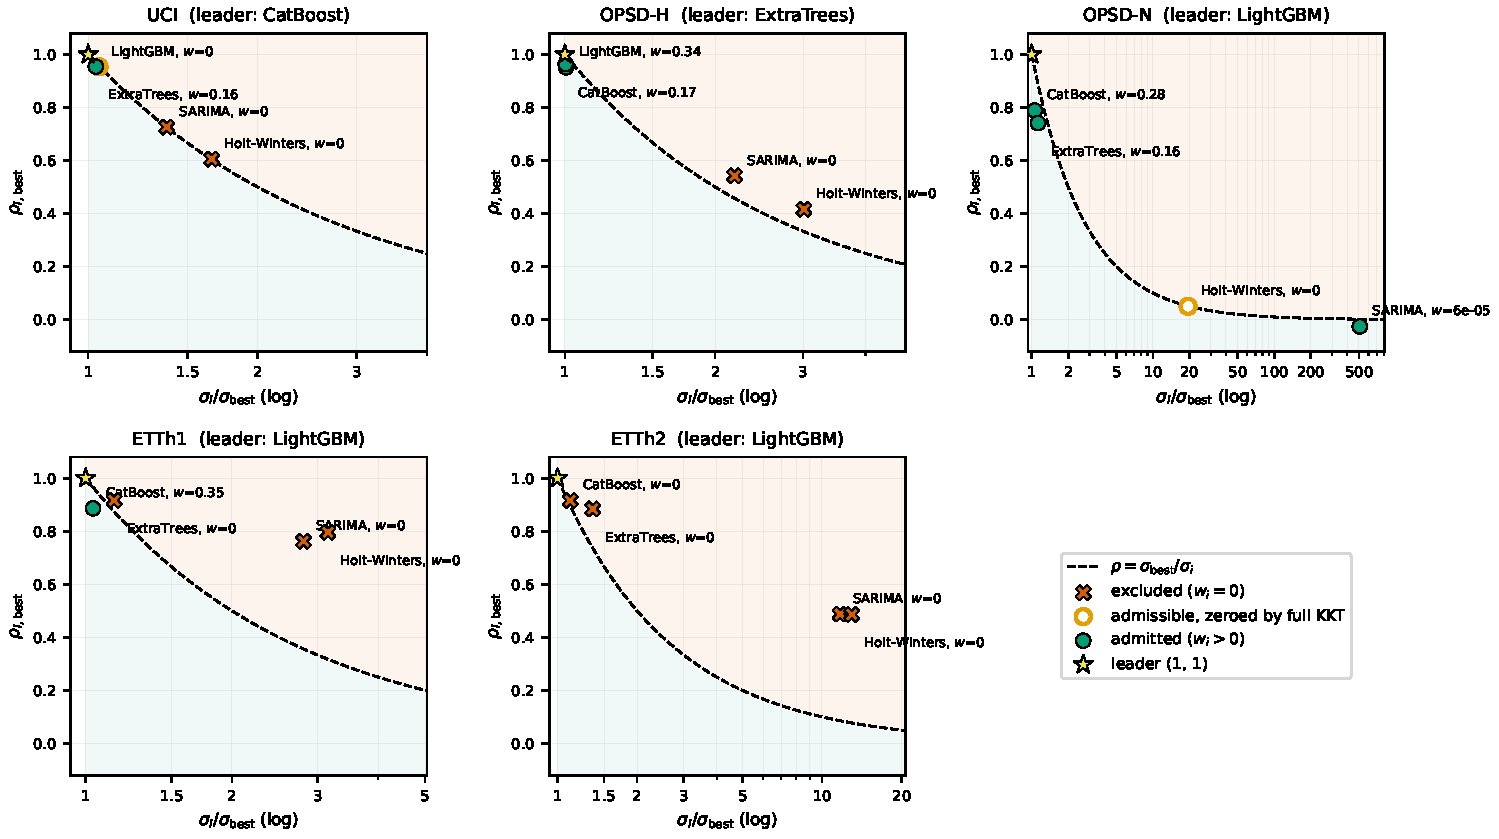
\includegraphics[width=0.9\textwidth]{fig2_kkt_boundary.pdf}
\caption{The exclusion boundary of Proposition~\ref{prop:boundary}, one panel per dataset. Each point is one CSE member, placed by its validation error-scale ratio to the leader (horizontal, logarithmic) and its uncentred error correlation with the leader (vertical); the dashed curve is $\rho = \sigma_{\mathrm{best}}/\sigma_i$ and the star is the leader. Filled circles received positive weight, crosses are excluded members with zero weight, and open circles are admissible members zeroed by the full KKT system. No member above the curve was admitted on any dataset.}
\label{fig:boundary}
\end{figure*}

\subsection{The exclusion boundary predicts the pattern}
\label{sec:boundary}
For each dataset we extract every member's validation error scale $\sigma_i$ and its uncentred correlation $\rho_i$ with the leading member, and place it in the plane of scale ratio against correlation with the boundary of \eqref{eq:boundary}. Fig.~\ref{fig:boundary} is that diagram and Table~\ref{tab:agree} its tabular form.

In the main benchmark the screen behaves as a necessary condition. Of the \nNonLeading{} non-leading member-dataset pairs, \nExcluded{} fall on the excluded side and all \nExcluded{} received weight exactly zero; on no dataset did a member violating \eqref{eq:boundary} receive positive weight. Of the \nAdmissible{} admissible members, \nAdmPositive{} received positive weight. The \nAdmZero{} that did not (\collList) are the cases Remark~\ref{rem:generalK} covers: each lies within \collMaxGap{} of the boundary in $\rho$ or is closely collinear with an admitted member, and the full KKT residual $(\Sigma w^{\star})_i - \lambda$ is positive for each of them. We evaluated \eqref{eq:kkt} at the solution for all 25 members on all five datasets: every active member has a residual of zero to machine precision and every zeroed member a positive residual, so the five-member programme is solved exactly and the sparsity pattern is a property of the optimisation problem rather than of the solver. Cases in which the screen fails in the other direction appear only in the fold and pool experiments (Section~\ref{sec:sens}) and are of the kind Remark~\ref{rem:generalK} describes.

Corollary~\ref{cor:admission} is illustrated by the OPSD-N SARIMA point: its error scale is \sarimaOPSDNratio{} times the leader's, which would disqualify it under any accuracy-based heuristic, yet its error correlation with the leader is \sarimaOPSDNrho, below the threshold \sarimaOPSDNthr, and it is admitted with a weight that is positive but practically negligible. We note the limits of this example: with a correlation that close to zero, the admission is a consequence of the sign of a small number, and the weight it earns matters little to the blend. Holt-Winters on the same series sits just inside the boundary ($\rho = \hwOPSDNrho$ against \hwOPSDNthr) and is nevertheless zeroed by the full system, with a relative residual of \hwOPSDNkkt. The optimiser is not selecting good models; it is selecting error directions the blend does not already have.

The collapse is thus a property of the geometry of the simplex-constrained least-squares problem applied to members whose errors are highly correlated with the leader's and whose scales are larger. In this benchmark the classical members occupy that region, so they are the ones that vanish. Section~\ref{sec:sens} asks whether this depends on the pool and the split.

\subsection{Sensitivity to the member pool and to the split}
\label{sec:sens}
\begin{table*}[!tb]
\caption{Sensitivity of the collapse to the member pool, one-step protocol, exact simplex weights on the validation slice. Pools use the benchmark's standalone model configurations, so the ``paper five'' row is the same five families with slightly different hyper-parameters from the CSE of Table~\ref{tab:weights}. ``zeroed'' counts members with exactly zero weight, ``viol.'' counts members above the boundary that received weight, and ``gap'' is the blend's test RMSE relative to its best active member. On OPSD-N the standalone SARIMA and Holt-Winters fits are skipped for memory, as in the main benchmark, so each pool there has two fewer members.}
\label{tab:sens}
\centering
\scriptsize
\setlength{\tabcolsep}{4pt}
\begin{tabular}{llrrrrrrr}
\toprule
Data & Pool & $K$ & zeroed & tree mass & viol. & RMSE blend & RMSE best member & gap \\
\midrule
ETTh1 & paper five & 5 & 4 & 1.000 & 0 & 0.670 & 0.670 (ExtraTrees) & $+$0.0\% \\
ETTh1 & + XGBoost, RF & 7 & 5 & 1.000 & 0 & 0.663 & 0.666 (RandomForest) & $-$0.4\% \\
ETTh1 & + Ridge, Lasso, EN & 8 & 4 & 0.127 & 0 & 0.630 & 0.631 (Ridge) & $-$0.3\% \\
ETTh1 & + NLinear, DLinear & 7 & 6 & 1.000 & 0 & 0.670 & 0.670 (ExtraTrees) & $+$0.0\% \\
ETTh1 & eight tree models & 8 & 5 & 1.000 & 0 & 0.645 & 0.657 (QuantileLightGBM) & $-$1.8\% \\
ETTh1 & all 22 & 22 & 18 & 0.157 & 0 & 0.629 & 0.631 (Ridge) & $-$0.4\% \\
ETTh2 & paper five & 5 & 3 & 1.000 & 0 & 0.674 & 0.684 (ExtraTrees) & $-$1.5\% \\
ETTh2 & + XGBoost, RF & 7 & 4 & 1.000 & 0 & 0.676 & 0.684 (ExtraTrees) & $-$1.2\% \\
ETTh2 & + Ridge, Lasso, EN & 8 & 5 & 0.097 & 0 & 0.687 & 0.684 (ExtraTrees) & $+$0.5\% \\
ETTh2 & + NLinear, DLinear & 7 & 5 & 1.000 & 0 & 0.674 & 0.684 (ExtraTrees) & $-$1.5\% \\
ETTh2 & eight tree models & 8 & 4 & 1.000 & 0 & 0.676 & 0.684 (ExtraTrees) & $-$1.2\% \\
ETTh2 & all 22 & 22 & 19 & 0.095 & 0 & 0.688 & 0.700 (Ridge) & $-$1.7\% \\
\bottomrule
\end{tabular}

\end{table*}
\begin{table*}[!tb]
\caption{Expanding-window folds for the CSE, one-step protocol: training ends at 50, 60, 70 and 80\% of each series and the following 20\% block (or what remains) is scored. All five members are refit on every fold so each member's own test RMSE is available.}
\label{tab:folds}
\centering
\scriptsize
\setlength{\tabcolsep}{4pt}
\begin{tabular}{lrrrrrrrl}
\toprule
Data & train end & $n_{\mathrm{test}}$ & tree mass & zeroed & viol. & RMSE CSE & RMSE best member & best member \\
\midrule
UCI & 50\% & 1\,719 & 0.926 & 1 & 0 & 0.545 & 0.543 & CatBoost \\
UCI & 60\% & 1\,719 & 0.851 & 1 & 0 & 0.596 & 0.576 & CatBoost \\
UCI & 70\% & 1\,719 & 1.000 & 2 & 0 & 0.603 & 0.598 & CatBoost \\
UCI & 80\% & 1\,719 & 1.000 & 3 & 0 & 0.638 & 0.636 & CatBoost \\
OPSD-H & 50\% & 7\,059 & 1.000 & 3 & 0 & 2.407 & 2.399 & ExtraTrees \\
OPSD-H & 60\% & 7\,059 & 0.790 & 2 & 0 & 0.204 & 0.227 & ExtraTrees \\
OPSD-H & 70\% & 7\,059 & 0.872 & 1 & 0 & 0.233 & 0.204 & CatBoost \\
OPSD-H & 80\% & 7\,059 & 0.965 & 1 & 0 & 0.159 & 0.157 & CatBoost \\
OPSD-N & 50\% & 10\,046 & 1.000 & 2 & 0 & 596.2 & 614.6 & LightGBM \\
OPSD-N & 60\% & 10\,046 & 1.000 & 2 & 0 & 529.7 & 541.7 & LightGBM \\
OPSD-N & 70\% & 10\,046 & 1.000 & 2 & 0 & 534.8 & 551.1 & LightGBM \\
OPSD-N & 80\% & 10\,046 & 1.000 & 1 & 0 & 591.8 & 619.1 & LightGBM \\
ETTh1 & 50\% & 3\,450 & 0.977 & 2 & 0 & 0.943 & 0.892 & CatBoost \\
ETTh1 & 60\% & 3\,450 & 1.000 & 3 & 0 & 0.992 & 1.000 & LightGBM \\
ETTh1 & 70\% & 3\,450 & 0.999 & 2 & 0 & 0.902 & 0.874 & LightGBM \\
ETTh1 & 80\% & 3\,450 & 1.000 & 3 & 0 & 0.672 & 0.681 & CatBoost \\
ETTh2 & 50\% & 3\,450 & 0.993 & 0 & 1 & 0.773 & 0.788 & LightGBM \\
ETTh2 & 60\% & 3\,450 & 1.000 & 3 & 0 & 0.899 & 0.882 & LightGBM \\
ETTh2 & 70\% & 3\,450 & 1.000 & 3 & 0 & 0.985 & 0.977 & LightGBM \\
ETTh2 & 80\% & 3\,450 & 1.000 & 4 & 0 & 0.704 & 0.704 & LightGBM \\
\bottomrule
\end{tabular}

\end{table*}
Two experiments test whether the collapse is an artefact of the five chosen members or of the single split. Table~\ref{tab:sens} stacks six different pools on the simplex: the paper's five families, the same five plus XGBoost and Random-Forest, plus three regularised linear models, plus the tuned NLinear and DLinear, the eight tree and boosting models alone, and every standalone model in the benchmark. Table~\ref{tab:folds} refits the CSE on four expanding windows per series. Across the \sensRows{} pool-dataset combinations the screen is violated \sensViolTimes, and at least one member receives exactly zero weight in \nSensAnyZero{} of them (the exception is \sensNoZeroDesc). Tree members hold the majority of the mass in \nSensHighTree{} of the \sensRows{} cases. In the remaining \nSensLowTree{} the mass moves to a member the CSE does not contain (\sensLowTreeList): the solver follows the validation leader, and on the ETT series the regularised linear models on lagged features are competitive with the trees one step ahead (Table~\ref{tab:main}). With every standalone model offered (\sensAllK, or \sensAllKMin{} on OPSD-N), the solver zeroes between \sensAllZeroMin{} and \sensAllZeroMax{} of them and keeps between \sensAllActiveMin{} and \sensAllActiveMax{} (\sensAllDesc). What persists under every pool is the collapse onto a handful of members with exact zeros elsewhere; the identity of the survivors is a property of the pool. The blend's test RMSE relative to its best active member ranges from \sensGapMin\% to \sensGapMax\%, and is lower than the best member in \sensGapBetter{} of \sensRows{} cases. Across the \foldRows{} folds the screen is violated \foldViolTimes, the tree mass never falls below \foldTreeMassMin, and the CSE is better than its best member on \foldBetter{} folds and worse on \foldWorse{}, by \foldGapMin\% to \foldGapMax\%. Violations of the screen on the folds: \foldViolDesc. Such cases arise when other active members cancel part of the admitted member's error, the mechanism of Remark~\ref{rem:generalK}; where the member sits near zero correlation the screen is decided by the sign of a small number and the admitted weight is negligible. The collapse onto few members, and the small and sign-varying gain of the blend over its best member, do not depend on the choice of five members or on the position of the split; which members survive does.

\subsection{Rolling-origin horizon results}
\label{sec:horizon}
The lower blocks of Table~\ref{tab:family} give the mean rank at each horizon, by model and by family. The pattern predicted by \eqref{eq:ar1} is visible: tree and boosting models hold mean rank \ranktreeHOne{} at $h = 1$ and drift to \ranktreeHTwoFour{} at $h = 24$, the lightweight linear models move the other way from \rankliteHOne{} to \rankliteHTwoFour, and the lagged linear family stays close to flat (\ranklinHOne{} at $h=1$, \ranklinHTwoFour{} at $h=24$). The CSE sits at mean rank \rankcseHOnemodel{} at $h = 1$, behind \bestRankHOne{} (\bestRankHOneVal), and falls to \rankcseHTwoFourmodel{} at $h = 24$, tracking its tree members. Per dataset the reversal is complete: at $h = 24$ the best models are \winnersHTwoFour, whereas at $h = 1$ the winners are \winnersHOne, \ifnum\nTreeWinnersHOne=5 a clean sweep for trees\else trees on \nTreeWinnersHOne{} of the five series\fi. The tree advantage is horizon-conditional, and it is gone by one day ahead.

\begin{table*}[!tb]
\caption{Diebold-Mariano test of the CSE against the best model per dataset and protocol on the fixed split, Holm adjusted, with both effect sizes; negative statistics favour the reference. The last two columns count the models that leader beats at the 5\% level and those it cannot be separated from.}
\label{tab:dm}
\centering
\scriptsize
\setlength{\tabcolsep}{4pt}
\begin{tabular}{lllrrrrcllc}
\toprule
Data & Protocol & Best model & RMSE (best) & RMSE (CSE) & DM stat & $p_{\mathrm{adj}}$ & $d$ / $\delta$ & Verdict & Beats & Ties \\
\midrule
UCI & one-step & ExtraTrees & 0.632 & \pending{0.639} & \pending{$-$1.55} & \pending{0.383} & \pending{$-$0.021 / $-$0.001} & \pending{tie} & 17 / 22 & 5 \\
UCI & recursive & SARIMA & 0.889 & \pending{1.108} & \pending{$-$11.13} & \pending{$< 10^{-4}$} & \pending{$-$0.372 / $-$0.222} & \pending{CSE worse} & 21 / 22 & 1 \\
OPSD-H & one-step & QuantileLightGBM & 0.156 & \pending{0.159} & \pending{$-$2.04} & \pending{0.041} & \pending{$-$0.301 / $-$0.203} & \pending{CSE worse} & 22 / 22 & 0 \\
OPSD-H & recursive & NaiveDrift & 0.175 & \pending{0.560} & \pending{$-$9.11} & \pending{$< 10^{-4}$} & \pending{$-$0.546 / $-$0.719} & \pending{CSE worse} & 22 / 22 & 0 \\
OPSD-N & one-step & \textbf{CSE (ours)} & -- & -- & -- & -- & -- & CSE is best & 18 / 18 & 0 \\
OPSD-N & recursive & XGBoost & 3\,756 & \pending{4\,373} & \pending{$-$29.54} & \pending{$< 10^{-4}$} & \pending{$-$0.461 / $-$0.102} & \pending{CSE worse} & 18 / 18 & 0 \\
ETTh1 & one-step & Ridge & 0.631 & 0.672 & $-$6.45 & $< 10^{-4}$ & $-$0.130 / $-$0.052 & CSE worse & 20 / 22 & 2 \\
ETTh1 & recursive & RandomForest & 2.880 & 3.529 & $-$12.62 & $< 10^{-4}$ & $-$0.213 / $-$0.129 & CSE worse & 22 / 22 & 0 \\
ETTh2 & one-step & ExtraTrees & 0.684 & 0.704 & $-$2.48 & 0.066 & $-$0.050 / $-$0.020 & tie & 17 / 22 & 5 \\
ETTh2 & recursive & LightGBM & 6.735 & 6.735 & $+$0.00 & 1.000 & -- / $+$0.000 & identical & 21 / 22 & 1 \\
\bottomrule
\end{tabular}

\end{table*}

\begin{figure}[!t]
\centering
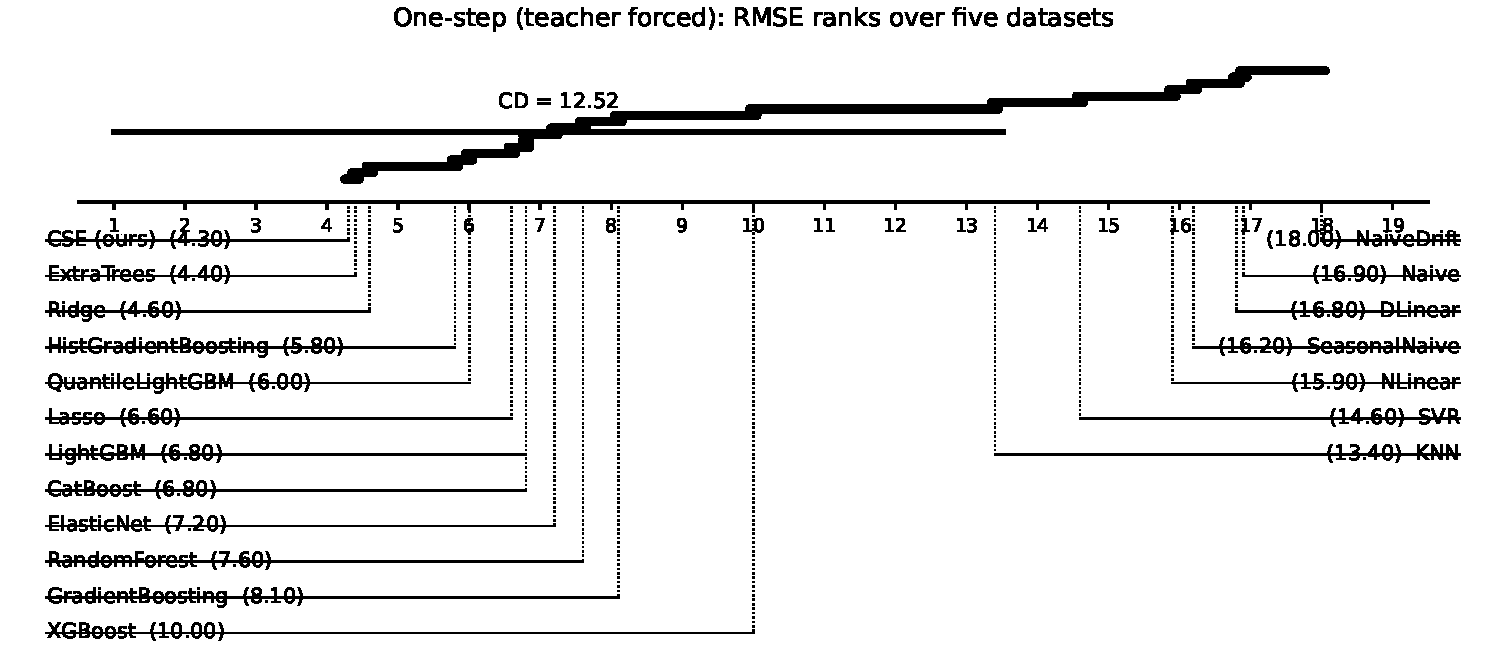
\includegraphics[width=\columnwidth]{fig3_cd_diagrams_one_step.pdf}\\[2pt]
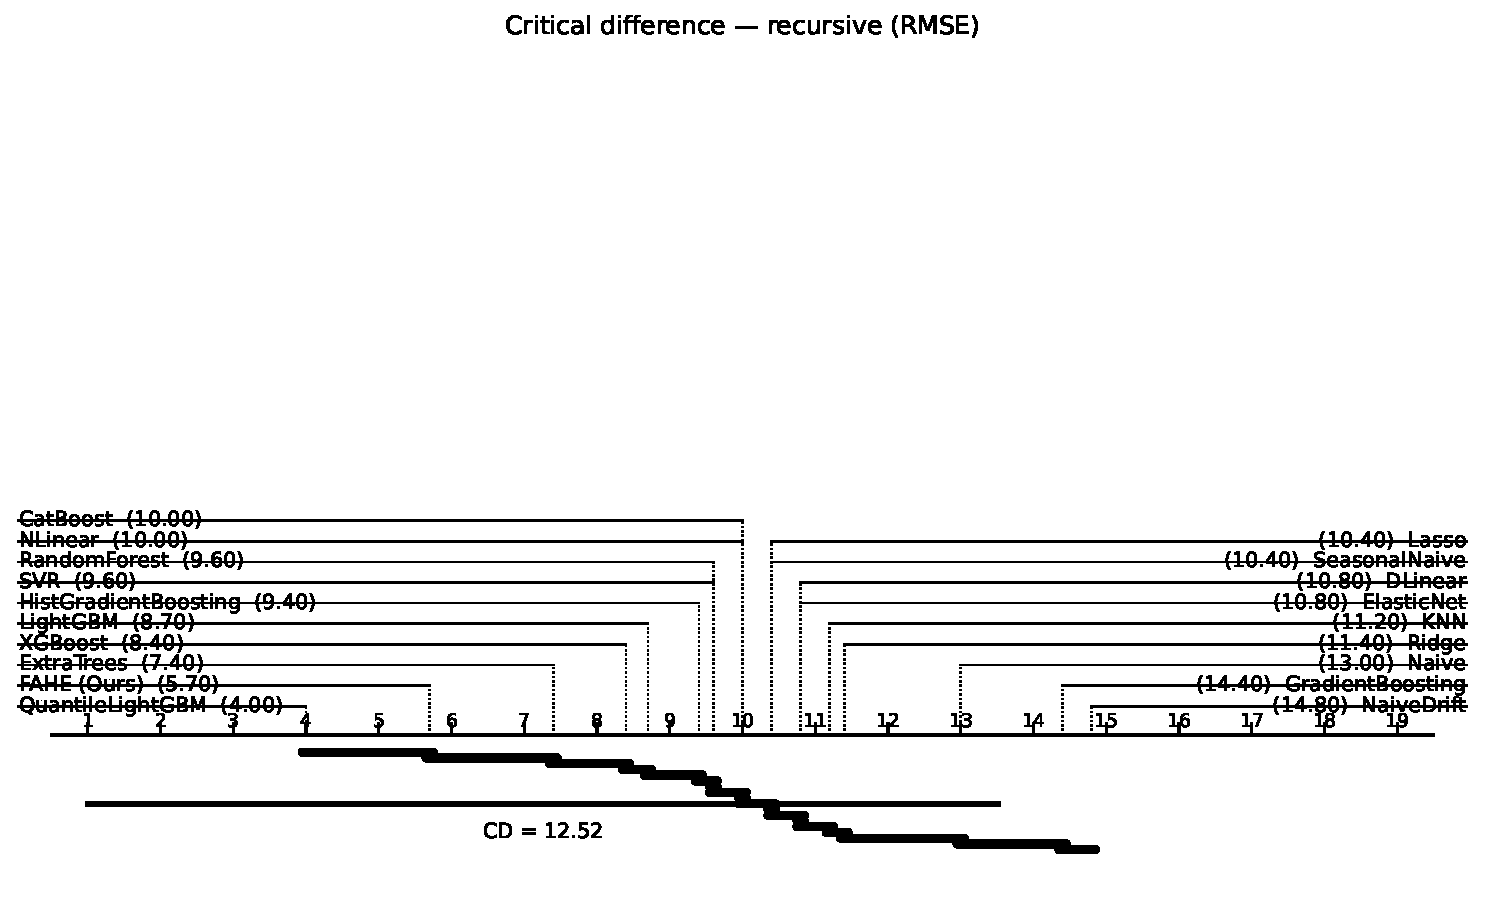
\includegraphics[width=\columnwidth]{fig3_cd_diagrams_recursive.pdf}
\caption{Nemenyi critical-difference diagrams over five datasets, RMSE ranks, one-step (top) and recursive (bottom). Models joined by a bar are not significantly different at the 5\% level.}
\label{fig:cd}
\end{figure}

\subsection{Statistical significance}
\label{sec:sig}
Table~\ref{tab:dm} tests the ensemble against the best model on each dataset and protocol, its last two columns showing how decisive each leader is against the rest of the field. One step ahead the CSE wins on \winListOne, where it is the reference and beats all \nBeatsOPSDDEtotalOne{} other models after Holm correction; it ties on \tieClausesOne; and it loses on \lossClausesOne. Under recursion it loses on \nLossRec{} datasets and is identical to \identModelETThTwoRec{} on \identListRec, where its weight sits entirely on that member. This is the answer to RQ2 and it is largely negative: a convex blend of five heterogeneous members does not reliably beat its strongest member, and when the collapse is complete it cannot, by construction.

The ordering by RMSE gap and the ordering by significance need not agree. \orderingNoteOne{} The Diebold-Mariano statistic weighs the mean loss differential against its own variance, whereas RMSE is driven by the tails, so a small but persistent gap is easier to detect than a larger one carried by a few hours. The effect sizes matter alongside the $p$-values. Where the CSE loses on ETTh1 one step ahead, $d = \dmETThOneOned$ and $\delta = \dmETThOneOnedelta$: statistically unambiguous, practically small. Where it loses on OPSD-H recursively, $d = \dmOPSDDEhouseholdRecd$ and $\delta = \dmOPSDDEhouseholdRecdelta$, a large effect and a worse forecaster. Reporting only $p$-values would have hidden that distinction, and reporting only RMSE would have hidden both. On the operational scale, the one-step differences among the leading tree models, the quantile booster and the CSE are a few percent of RMSE on every series, which is within the range a utility would attribute to feature or calibration changes rather than to model class.

The Friedman result is the single most consequential number here. Under teacher forcing the null of equal accuracy across the \friedKOne{} common models is rejected decisively ($\chi^2 = \friedChiOne$, $p \friedPOne$); under the recursive protocol, on the same datasets and models, it cannot be rejected ($\chi^2 = \friedChiRec$, $p \friedPRec$). With five datasets the Friedman test has limited power, so the second result is weak evidence of equality; it is nevertheless a direct statement that the discriminative power of the benchmark, the very thing a leaderboard is supposed to supply, comes mostly from supplying true lagged actuals at test time. Fig.~\ref{fig:cd} shows this as critical-difference diagrams: the one-step diagram separates the field into recognisable groups, the recursive diagram connects almost everything into one clique.

\subsection{Tuned baselines and cost}
\label{sec:cost}
\begin{table}[!t]
\caption{Tuned NLinear and DLinear configurations (Optuna search over lookback, ridge penalty, kernel size and clipping quantile, objective one-step validation RMSE) and their test scores.}
\label{tab:tuned}
\centering
\scriptsize
\setlength{\tabcolsep}{4pt}
\begin{tabular}{llrrrrr}
\toprule
Data & Model & Lookback & Clip $q$ & Val RMSE & Test RMSE & Test $R^2$ \\
\midrule
UCI & NLinear & 336 & 0.99 & 0.840 & 0.950 & 0.187 \\
UCI & DLinear & 336 & 0.95 & 0.838 & 0.950 & 0.188 \\
OPSD-H & NLinear & 48 & 0.995 & 0.364 & 0.176 & $-$0.014 \\
OPSD-H & DLinear & 336 & 0.975 & 0.223 & 0.208 & $-$0.411 \\
OPSD-N & NLinear & 336 & 0.975 & 8\,370 & 6\,695 & 0.537 \\
OPSD-N & DLinear & 336 & 0.975 & 8\,267 & 6\,616 & 0.548 \\
ETTh1 & NLinear & 96 & 0.95 & 5.756 & 6.640 & $-$2.737 \\
ETTh1 & DLinear & 24 & 0.95 & 2.754 & 7.835 & $-$4.204 \\
ETTh2 & NLinear & 336 & 0.99 & 11.72 & 22.52 & $-$3.503 \\
ETTh2 & DLinear & 24 & 0.95 & 7.510 & 24.26 & $-$4.225 \\
\bottomrule
\end{tabular}

\end{table}
\begin{table}[!t]
\caption{Training time of the CSE in seconds when only the members with positive weight are refit on the full training partition, against the same fit with every member refit (the 80\% expanding-window fold, identical training data). Forecasts are identical in both cases. Times are single wall-clock runs on one laptop.}
\label{tab:refit}
\centering
\scriptsize
\setlength{\tabcolsep}{4pt}
\begin{tabular}{lrrrp{3.1cm}}
\toprule
Data & active (s) & full (s) & saving & members not refit \\
\midrule
UCI & 36 & 56 & 36\% & SARIMA, Holt-Winters, LightGBM \\
OPSD-H & 71 & 134 & 47\% & SARIMA, Holt-Winters \\
OPSD-N & 496 & 479 & none & Holt-Winters \\
ETTh1 & 62 & 132 & 53\% & SARIMA, Holt-Winters, ExtraTrees \\
ETTh2 & 46 & 76 & 38\% & SARIMA, Holt-Winters, CatBoost, ExtraTrees \\
\bottomrule
\end{tabular}

\end{table}
\begin{table}[!t]
\caption{Training time in seconds, one-step protocol, single CPU core. The CSE row includes the validation fits of all five members and the refit of the members with positive weight only.}
\label{tab:cost}
\centering
\scriptsize
\setlength{\tabcolsep}{4pt}
\begin{tabular}{lrrrrr}
\toprule
Model & UCI & OPSD-H & OPSD-N & ETTh1 & ETTh2 \\
\midrule
SARIMA & 17.1 & 334.0 & -- & 66.6 & 28.3 \\
Holt-Winters & 0.331 & 6.216 & -- & 9.816 & 31.7 \\
ExtraTrees & 1.590 & 6.921 & 10.6 & 3.486 & 3.396 \\
LightGBM & 2.474 & 1.994 & 1.904 & 1.996 & 2.840 \\
CatBoost & 6.831 & 7.437 & 8.312 & 7.807 & 7.681 \\
HistGradientBoosting & 1.069 & 0.141 & 1.272 & 0.364 & 0.923 \\
NLinear & 0.012 & 0.007 & 0.052 & 0.004 & 0.029 \\
DLinear & 0.365 & 0.947 & 1.532 & 0.358 & 0.327 \\
\textbf{CSE (ours)} & 36.1 & 261.0 & 496.1 & 61.7 & 46.5 \\
\bottomrule
\end{tabular}

\end{table}
Both lightweight linear models were tuned with reversible instance normalisation \cite{r30}, robust clipping and an Optuna \cite{r31} search (Table~\ref{tab:tuned}). On UCI, DLinear reaches \dlinearUCI~kW, in line with NLinear and SARIMA. On ETT both remain weak ($R^2$ between \liteRTwoETTmin{} and \liteRTwoETTmax), and we report that rather than dropping the rows. The objective here was one-step validation RMSE, not the long-horizon regime these architectures were designed for, and the lookbacks selected on ETTh1 are far shorter than the 336-step windows of the original setting. That is a limitation of this benchmark's treatment of them, not evidence about the architectures.

Accuracy is not matched by cost (Table~\ref{tab:cost}). HistGradientBoosting trains in under \hgbTimeMax~s on every dataset and is within a few percent of the leaders one step ahead, while the CSE costs \cseTimeMin~s to \cseTimeMax~s, between \costRatioLgbMin{} and \costRatioLgbMax{} times a single LightGBM fit, because it fits five members on the validation window and then refits the active ones. The KKT analysis reduces that cost directly. A member with zero weight never enters the blend, so skipping its second fit changes nothing in the forecasts. Table~\ref{tab:refit} compares the ensemble's training time with and without that step: the saving is \refitSaveMin\% to \refitSaveMax\% on \nRefitSaved{} series and negligible on \refitNoSaveList, where the only member skipped is the cheap Holt-Winters fit and the expensive SARIMA member keeps a weight of \wSarimaOPSDNsci{} and must be refit. Removing such a member by a weight threshold would recover the saving there at no visible cost in accuracy, but we report the exact solution. The same information is available before the second fit on any series, because the weights are computed from the validation errors alone. For a deployment that gains nothing over a single boosted model, and on four of five datasets it gains nothing, the remaining cost is still hard to justify; the diagnosis at least tells the practitioner so in advance.

\section{Discussion}
\subsection{Answers to the research questions}
\label{sec:answers}
\textbf{RQ1.} No family dominates unconditionally: trees lead \nTreeWinsOne{} of five datasets one step ahead (\treeWinsOneList), the tree-dominated CSE leads \winListOne, \linearWinsOneModel{} on lagged features wins \linearWinsOneList, and under recursion \bestRecUCI{} leads UCI and \bestRecOPSDDEhousehold{} leads OPSD-H. Tree ensembles share the one-step regime with the lagged linear models on these series, which is far narrower than the usual claim.

\textbf{RQ2.} No, not reliably. The CSE has the best one-step mean rank and beats all \nBeatsOPSDDEtotalOne{} other models on OPSD-N, but elsewhere it ties \tiesTimesOne{} and loses \lossTimesOne, and under recursion it loses \lossTimesRec{} and is identical to a single member \identTimesRec. On the folds and the alternative pools the gain over the best member is small and changes sign. It is a defensible default, not an improvement.

\textbf{RQ3.} Yes, from the full KKT system, which holds for all 25 members and is exact; the pairwise screen agrees with it on \nAgree{} of \nNonLeading{} pairs in the main benchmark, is never violated there in the excluded direction, and fails \foldViolTimes{} across the folds and \sensViolTimes{} across the pools, in each case for a member on the boundary or with a negligible weight. The collapse itself does not depend on the member pool or the split.

\textbf{RQ4.} A substantial share of the ranking is protocol, not capacity: Friedman rejects equal accuracy one step ahead ($p \friedPOne$) and cannot reject it under recursion ($p \friedPRec$), tree models degrade by median factors of \treeDegMin{} to \treeDegMax{} while classical and direct models are unchanged, \tauOPSDHClause, and the tree advantage disappears by $h = 24$.

\subsection{What this means in practice}
Three recommendations follow from the evidence. First, if you intend to combine forecasts, compute the members' validation error moments before you fit the weights. Fig.~\ref{fig:boundary} can be drawn without touching the test set and tells you which members the optimiser will discard; if every candidate sits above the boundary, the combination will reproduce your best model at several times the training cost, and the honest move is to ship the best model. Where some members are admitted, refit only those. Second, the constraint set is doing more work than the weights. Non-negativity is what makes the collapse legible: an unconstrained blend would have given the classical members small negative coefficients and reported a marginal improvement that would not survive out of sample. Third, report the protocol as prominently as the metric. A one-step leaderboard on a residential series measures interpolation given the previous hour's true consumption. That is a real operational task, for example behind-the-meter control with metering feedback, but it is not the day-ahead task, and the two rankings can be almost uncorrelated.

The mechanism behind both findings is the same. Supervised learners scored one step ahead receive the true lagged actual at every test point, and on hourly load the lag-1 value alone explains most of the variance. Trees exploit it, correlate strongly with the target, dominate the leaderboard, and by \eqref{eq:kkt} absorb all of the stacking weight. Remove the true lag, as recursion does, and their advantage collapses to the level of models that never had it.

\section{Limitations and Threats to Validity}
\label{sec:limits}
\textbf{No Transformer baselines.} The code includes Autoformer, FEDformer, Informer, iTransformer and PatchTST, but the artefacts here were produced on CPU and contain no rows for them, so every deep-model statement concerns tuned lightweight linear architectures only. Zeng \emph{et al.} \cite{r15} suggest those are a reasonable proxy, but that is an argument from the literature, not evidence from this benchmark, and the one-step leaderboard should be read with that gap in mind.

\textbf{Lightweight linear models are weak on ETT.} NLinear and DLinear reach negative $R^2$ on both ETT series even after tuning; a study focused on them would use a horizon-aggregated objective.

\textbf{Reduced model set on OPSD-N.} Nineteen rather than 23 models appear on the national load series, since the standalone heavy classical fits exceeded the memory budget at 50\,400 observations. The CSE keeps its internal SARIMA and Holt-Winters branches, so the collapse analysis is unaffected, but the classical family is under-represented in that column of Table~\ref{tab:main}.

\textbf{Two protocols, one seed.} The fixed-split recursive protocol rolls out over thousands of hours and is a stress test rather than an operating condition; the rolling-origin tables are the operational comparison, and the fold experiment covers the split for the CSE only. Repeated seeds and a moving-block bootstrap over test blocks would give confidence intervals on the leaderboard itself.

\textbf{The pairwise boundary is not the full KKT system.} Proposition~\ref{prop:boundary} is exact for $K = 2$ and only a screen for $K = 5$, with counterexamples in both directions (Remark~\ref{rem:generalK}); we verified the full system numerically on every dataset rather than characterising its active set in closed form as a function of $\Sigma$, which remains open for stacking.

\textbf{Frequency-aware ensembles remain untested.} The most promising route to an ensemble that does not collapse is to build members satisfying \eqref{eq:boundary} by design, for example by decomposing the signal into disjoint frequency bands and fitting a specialist to each, so member errors are approximately orthogonal. Whether that beats plain boosting is open and directly testable with the framework released here.

\section{Conclusion}
We reported a controlled benchmark of up to 23 forecasters on five hourly energy series under two protocols, with rolling-origin horizon tables, a full significance suite and a KKT analysis of simplex-constrained combination. The central finding holds on all five datasets: a convex stacking ensemble collapses onto tree learners, the full KKT system of the fitted programme accounts for every zero, the classical pairwise screen $\rho_i \geq \sigma_{\mathrm{best}}/\sigma_i$ predicts them on \nAgree{} of \nNonLeading{} pairs with no violation in the excluded direction, and the pattern survives changes of member pool and of split. The diagnosis has one direct use: a zeroed member need not be refit, which cut the ensemble's training time by \refitSaveMin\% to \refitSaveMax\% on \nRefitSavedWord{} of the five series without changing a forecast.

The negative results matter as much. The ensemble does not reliably beat its strongest member, and the leaderboard that motivates ensembles is largely protocol-generated, since equal accuracy across \friedKOne{} models is rejected under teacher forcing and cannot be rejected under a recursive protocol on the same data. For practitioners: draw the error-geometry diagram before fitting combination weights, refit only what the weights keep, evaluate every family under the protocol you will deploy, and treat a one-step leaderboard as a statement about the availability of recent truth rather than about model capacity.

\appendices
\section{Per-Dataset Rolling-Origin Results}
Table~\ref{tab:app} gives rolling-origin test RMSE at each horizon for every model, averaged over 24 forecast origins per dataset.
\begin{table*}[!tb]
\caption{Rolling-origin test RMSE by horizon $h$, 24 origins per dataset, best per column in bold. Units: kW (UCI, OPSD-H), MW (OPSD-N), degrees (ETT).}
\label{tab:app}
\centering
\tiny
\setlength{\tabcolsep}{1.6pt}
\begin{tabular}{lrrrrrrrrrrrrrrrrrrrrrrrrr}
\toprule
& \multicolumn{5}{c}{UCI} & \multicolumn{5}{c}{OPSD-H} & \multicolumn{5}{c}{OPSD-N} & \multicolumn{5}{c}{ETTh1} & \multicolumn{5}{c}{ETTh2} \\
\cmidrule(lr){2-6}\cmidrule(lr){7-11}\cmidrule(lr){12-16}\cmidrule(lr){17-21}\cmidrule(lr){22-26}
Model & 1 & 3 & 6 & 12 & 24 & 1 & 3 & 6 & 12 & 24 & 1 & 3 & 6 & 12 & 24 & 1 & 3 & 6 & 12 & 24 & 1 & 3 & 6 & 12 & 24 \\
\midrule
Naive & 0.780 & 1.371 & 1.593 & 1.431 & 1.034 & 0.156 & 0.150 & 0.189 & 0.298 & 0.314 & 2934 & 6541 & 11420 & 14117 & 6964 & 0.603 & 1.028 & 1.639 & 1.606 & 1.811 & 1.745 & 4.126 & 6.669 & 6.988 & \textbf{3.822} \\
NaiveDrift & 0.780 & 1.372 & 1.593 & 1.431 & 1.031 & 0.156 & 0.150 & 0.189 & 0.298 & 0.314 & 2934 & 6541 & 11420 & 14118 & 6965 & 0.603 & 1.028 & 1.642 & 1.613 & 1.823 & 1.745 & 4.127 & 6.670 & 6.993 & 3.827 \\
SeasonalNaive & 0.995 & 1.292 & 1.307 & 1.103 & 1.034 & 0.272 & 0.080 & 0.273 & 0.309 & 0.314 & 5438 & 5256 & 6186 & 7586 & 6964 & 3.012 & 2.717 & 2.265 & 2.189 & 1.811 & 5.733 & 6.408 & 5.751 & 4.574 & \textbf{3.822} \\
NLinear & 0.550 & 0.944 & 0.967 & 0.723 & 0.636 & 0.128 & 0.077 & 0.160 & 0.228 & 0.241 & 832.91 & 1430 & 1834 & 4166 & 2968 & 0.573 & \textbf{0.889} & 1.290 & 1.337 & 1.624 & 1.380 & 2.711 & 3.665 & \textbf{3.176} & 3.943 \\
DLinear & 0.541 & 0.933 & 0.976 & 0.711 & \textbf{0.625} & 0.136 & 0.080 & \textbf{0.146} & 0.245 & 0.219 & 838.68 & 1435 & 1827 & 4167 & 2935 & 0.580 & 0.897 & 1.434 & 1.562 & 1.593 & 1.352 & 2.779 & 4.028 & 4.145 & 4.006 \\
Ridge & 0.579 & 0.988 & 0.973 & 0.682 & 0.740 & 0.143 & 0.123 & 0.240 & 0.263 & 0.302 & 1076 & 1731 & 3111 & 4257 & 4494 & 0.573 & 1.011 & 1.387 & 1.450 & 1.530 & 1.338 & 2.583 & 3.606 & 3.261 & 3.931 \\
Lasso & 0.567 & 1.002 & 0.994 & 0.662 & 0.722 & 0.156 & 0.125 & 0.238 & 0.271 & 0.291 & 1085 & 1763 & 3136 & 4265 & 4512 & 0.575 & 1.037 & 1.416 & 1.496 & \textbf{1.501} & 1.356 & 2.633 & 3.684 & 3.181 & 4.116 \\
ElasticNet & 0.572 & 0.996 & 0.986 & 0.667 & 0.721 & 0.153 & 0.123 & 0.239 & 0.268 & 0.293 & 1079 & 1622 & 3023 & 4284 & 4486 & 0.575 & 1.023 & 1.408 & 1.479 & 1.508 & 1.383 & 2.645 & 3.691 & 3.192 & 4.103 \\
KNN & 0.654 & 1.098 & 1.121 & \textbf{0.587} & 0.681 & 0.168 & 0.143 & 0.172 & 0.276 & 0.224 & 1829 & 1904 & 2182 & 3853 & 4203 & 2.431 & 2.158 & 2.594 & 2.373 & 3.211 & 2.753 & 4.767 & 6.772 & 5.974 & 7.015 \\
SVR & 0.587 & 0.935 & 0.963 & 0.627 & 0.711 & 0.153 & 0.136 & 0.181 & 0.239 & 0.226 & 7441 & 8149 & 9465 & 10034 & 8550 & 1.240 & 1.546 & 1.889 & 2.456 & 3.226 & 1.375 & 3.348 & 5.282 & 6.049 & 7.442 \\
RandomForest & 0.579 & 0.904 & \textbf{0.952} & 0.699 & 0.796 & 0.125 & 0.108 & 0.172 & 0.288 & 0.212 & 769.25 & 1318 & 1698 & 3873 & 2927 & \textbf{0.531} & 0.992 & 1.197 & \textbf{1.270} & 1.766 & 1.587 & 2.953 & 4.155 & 3.680 & 5.170 \\
ExtraTrees & 0.581 & 0.939 & 1.014 & 0.907 & 0.865 & 0.199 & 0.561 & 0.226 & 0.262 & 0.246 & 758.24 & 1183 & 1385 & 3634 & \textbf{2508} & 0.589 & 0.941 & \textbf{1.164} & 1.353 & 1.841 & 1.501 & 2.823 & 3.980 & 3.448 & 4.659 \\
GradientBoosting & 0.547 & 0.956 & 1.037 & 0.827 & 0.951 & \textbf{0.109} & 0.086 & 0.166 & 0.413 & \textbf{0.206} & 1181 & 1475 & 1928 & 4057 & 4115 & 0.612 & 1.043 & 1.630 & 1.869 & 2.003 & 1.582 & 2.972 & 4.248 & 3.413 & 5.115 \\
HistGradientBoosting & 0.592 & 0.925 & 1.096 & 0.822 & 0.831 & 0.177 & 0.198 & 0.204 & 0.263 & 0.223 & 762.86 & 1224 & 1589 & 3752 & 2955 & 0.599 & 1.065 & 1.324 & 1.653 & 2.246 & 1.521 & 2.928 & 4.199 & 3.796 & 5.227 \\
XGBoost & 0.546 & 0.961 & 1.085 & 0.904 & 0.989 & 0.167 & 0.584 & 0.236 & 0.309 & 0.292 & \textbf{615.57} & \textbf{1007} & \textbf{1265} & 3600 & 3274 & 0.544 & 1.191 & 1.589 & 1.755 & 2.162 & 1.349 & \textbf{2.554} & 3.863 & 3.656 & 4.865 \\
LightGBM & 0.599 & 1.005 & 1.145 & 0.940 & 0.922 & 0.163 & 0.478 & 1.533 & 0.962 & 1.547 & 669.20 & 1083 & 1426 & 3505 & 3142 & 0.594 & 1.184 & 1.548 & 1.823 & 2.642 & \textbf{1.285} & 2.616 & 3.934 & 3.748 & 5.319 \\
CatBoost & \textbf{0.527} & \textbf{0.892} & 0.986 & 0.861 & 0.922 & 0.111 & 0.112 & 0.179 & 0.226 & 0.242 & 716.01 & 1116 & 1468 & 3575 & 2709 & 0.713 & 1.038 & 1.212 & 1.925 & 2.695 & 1.376 & 2.813 & 4.747 & 4.551 & 4.997 \\
QuantileLightGBM & 0.543 & 0.925 & 0.996 & 0.662 & 0.661 & 0.111 & \textbf{0.075} & 0.153 & 0.240 & 0.233 & 973.21 & 1489 & 1721 & 3848 & 4114 & 0.593 & 1.036 & 1.289 & 1.653 & 1.973 & 1.509 & 2.560 & \textbf{3.533} & 3.594 & 4.932 \\
\textbf{CSE (ours)} & 0.539 & 0.897 & 0.969 & 0.856 & 0.825 & 0.128 & 0.139 & 0.186 & \textbf{0.224} & 0.235 & 676.09 & 1048 & 1293 & \textbf{3489} & 2821 & 0.606 & 1.121 & 1.445 & 1.676 & 2.267 & \textbf{1.285} & 2.616 & 3.934 & 3.748 & 5.319 \\
\bottomrule
\end{tabular}

\end{table*}

\section*{Reproducibility}
Every table, figure and inline number is regenerated by script from the released artefact directory (\texttt{leaderboards.csv}, \texttt{cse\_diagnostics/}, \texttt{multistep\_rolling/}, \texttt{significance/}, \texttt{tables/}). Seeds are fixed at 42 and no value was transcribed by hand. The code and the artefacts are released under the Apache License 2.0 at \url{https://github.com/aksingh1608/kkt-forecast-combination}; the five series are public and remain under their own upstream terms, which the repository documents together with the retrieval and cleaning steps.

\begin{thebibliography}{33}
\bibitem{r1} T. Hong et al., ``Energy forecasting: A review and outlook,'' \emph{IEEE Open Access J. Power Energy}, vol. 7, pp. 376--388, 2020.
\bibitem{r2} C. Kuster, Y. Rezgui, and M. Mourshed, ``Electrical load forecasting models: A critical systematic review,'' \emph{Sustain. Cities Soc.}, vol. 35, pp. 257--270, 2017.
\bibitem{r3} M. Peplinski et al., ``A machine learning framework to estimate residential electricity demand based on smart meter electricity, climate, building characteristics, and socioeconomic datasets,'' \emph{Appl. Energy}, vol. 357, p. 122413, 2024.
\bibitem{r4} R. Ramanathan and C. W. J. Granger, ``Improved methods of combining forecasts,'' \emph{J. Forecast.}, vol. 3, no. 2, pp. 197--204, 1984.
\bibitem{r5} P. V. B. Ramos, S. M. Villela, W. N. Silva, and B. H. Dias, ``Residential energy consumption forecasting using deep learning models,'' \emph{Appl. Energy}, vol. 350, p. 121705, 2023.
\bibitem{r6} R. J. Hyndman and G. Athanasopoulos, \emph{Forecasting: Principles and Practice}, 2nd ed. Melbourne, Australia: OTexts, 2018.
\bibitem{r7} L. Breiman, ``Random forests,'' \emph{Mach. Learn.}, vol. 45, no. 1, pp. 5--32, 2001.
\bibitem{r8} P. Geurts, D. Ernst, and L. Wehenkel, ``Extremely randomized trees,'' \emph{Mach. Learn.}, vol. 63, no. 1, pp. 3--42, 2006.
\bibitem{r9} T. Chen and C. Guestrin, ``XGBoost: A scalable tree boosting system,'' in \emph{Proc. 22nd ACM SIGKDD}, 2016, pp. 785--794.
\bibitem{r10} G. Ke et al., ``LightGBM: A highly efficient gradient boosting decision tree,'' in \emph{Adv. Neural Inf. Process. Syst.}, vol. 30, 2017.
\bibitem{r11} L. Prokhorenkova et al., ``CatBoost: Unbiased boosting with categorical features,'' in \emph{Adv. Neural Inf. Process. Syst.}, vol. 31, 2018.
\bibitem{r12} S. Makridakis, E. Spiliotis, and V. Assimakopoulos, ``M5 accuracy competition: Results, findings, and conclusions,'' \emph{Int. J. Forecast.}, vol. 38, no. 4, pp. 1346--1364, 2022.
\bibitem{r13} L. Semmelmann et al., ``The impact of heat pumps on day-ahead energy community load forecasting,'' \emph{Appl. Energy}, vol. 368, p. 123364, 2024.
\bibitem{r14} A. Das, W. Kong, R. Sen, and Y. Zhou, ``A decoder-only foundation model for time-series forecasting,'' in \emph{Proc. Int. Conf. Mach. Learn.}, 2024.
\bibitem{r15} A. Zeng, M. Chen, L. Zhang, and Q. Xu, ``Are Transformers effective for time series forecasting?'' in \emph{Proc. AAAI Conf. Artif. Intell.}, 2023, pp. 11121--11128.
\bibitem{r16} H. Zhou et al., ``Informer: Beyond efficient Transformer for long sequence time-series forecasting,'' in \emph{Proc. AAAI Conf. Artif. Intell.}, 2021, pp. 11106--11115.
\bibitem{r17} A. Timmermann, ``Forecast combinations,'' in \emph{Handbook of Economic Forecasting}, vol. 1, Amsterdam, The Netherlands: Elsevier, 2006, pp. 135--196.
\bibitem{r18} D. H. Wolpert, ``Stacked generalization,'' \emph{Neural Netw.}, vol. 5, no. 2, pp. 241--259, 1992.
\bibitem{r19} L. Breiman, ``Stacked regressions,'' \emph{Mach. Learn.}, vol. 24, no. 1, pp. 49--64, 1996.
\bibitem{r20} C. L. Lawson and R. J. Hanson, \emph{Solving Least Squares Problems}. Philadelphia, PA, USA: SIAM, 1995.
\bibitem{r21} S. Boyd and L. Vandenberghe, \emph{Convex Optimization}. Cambridge, U.K.: Cambridge Univ. Press, 2004.
\bibitem{r22} F. X. Diebold and R. S. Mariano, ``Comparing predictive accuracy,'' \emph{J. Bus. Econ. Statist.}, vol. 13, no. 3, pp. 253--263, 1995.
\bibitem{r23} D. Harvey, S. Leybourne, and P. Newbold, ``Testing the equality of prediction mean squared errors,'' \emph{Int. J. Forecast.}, vol. 13, no. 2, pp. 281--291, 1997.
\bibitem{r24} J. Dem\v{s}ar, ``Statistical comparisons of classifiers over multiple data sets,'' \emph{J. Mach. Learn. Res.}, vol. 7, pp. 1--30, 2006.
\bibitem{r25} N. Cliff, ``Dominance statistics: Ordinal analyses to answer ordinal questions,'' \emph{Psychol. Bull.}, vol. 114, no. 3, pp. 494--509, 1993.
\bibitem{r26} S. Holm, ``A simple sequentially rejective multiple test procedure,'' \emph{Scand. J. Statist.}, vol. 6, no. 2, pp. 65--70, 1979.
\bibitem{r27} L. J. Tashman, ``Out-of-sample tests of forecasting accuracy: An analysis and review,'' \emph{Int. J. Forecast.}, vol. 16, no. 4, pp. 437--450, 2000.
\bibitem{r28} Open Power System Data, ``Data package: Time series,'' 2020. [Online]. Available: \url{https://data.open-power-system-data.org/time_series/}
\bibitem{r29} G. H\'ebrail and A. B\'erard, ``Individual household electric power consumption data set,'' UCI Machine Learning Repository, 2012.
\bibitem{r30} T. Kim et al., ``Reversible instance normalization for accurate time-series forecasting against distribution shift,'' in \emph{Proc. Int. Conf. Learn. Represent.}, 2022.
\bibitem{r31} T. Akiba et al., ``Optuna: A next-generation hyperparameter optimization framework,'' in \emph{Proc. 25th ACM SIGKDD}, 2019, pp. 2623--2631.
\bibitem{r32} J. M. Bates and C. W. J. Granger, ``The combination of forecasts,'' \emph{Oper. Res. Quart.}, vol. 20, no. 4, pp. 451--468, 1969.
\bibitem{r33} P. Radchenko, A. L. Vasnev, and W. Wang, ``Too similar to combine? On negative weights in forecast combination,'' \emph{Int. J. Forecast.}, vol. 39, no. 1, pp. 18--38, 2023.
\end{thebibliography}

% Author biographies are requested at acceptance. Fill in and move above
% \end{document} when needed.
\iffalse
\begin{IEEEbiographynophoto}{Aryan Kumar Singh}
received the B.Tech.\ degree in computer science and engineering from Lovely Professional University, Punjab, India, in 2024. He is currently working toward the M.Sc.\ degree in artificial intelligence at the Berlin School of Business and Innovation, Berlin, Germany. His research interests include time-series forecasting, forecast combination, convex optimisation for machine learning and reproducible benchmarking for energy systems.
\end{IEEEbiographynophoto}
\fi
\end{document}
